%% Copyright (c) 2003,2004,2005  INRIA Sophia-Antipolis (France).
%% All rights reserved.
%%
%% This file is part of CGAL (www.cgal.org).
%% You can redistribute it and/or modify it under the terms of the GNU
%% General Public License as published by the Free Software Foundation,
%% either version 3 of the License, or (at your option) any later version.
%%
%% Licensees holding a valid commercial license may use this file in
%% accordance with the commercial license agreement provided with the software.
%%
%% This file is provided AS IS with NO WARRANTY OF ANY KIND, INCLUDING THE
%% WARRANTY OF DESIGN, MERCHANTABILITY AND FITNESS FOR A PARTICULAR PURPOSE.
%%
%% $URL$
%% $Id$
%% 
%%
%% Author(s)     : Menelaos Karavelas <mkaravel@iacm.forth.gr>


% +------------------------------------------------------------------------+
% | Reference manual page: Convex_hull_d_ref/intro.tex
% +------------------------------------------------------------------------+

%\clearpage
%\section{Reference Pages for dD Convex Hulls and Delaunay Triangulations}
\ccRefChapter{dD Convex Hulls and Delaunay Triangulations\label{chap:convex_hull_d_ref}}
\ccChapterAuthor{Susan Hert \and Michael Seel}

A subset $S \subseteq \R^3$ is convex if for any two points $p$ and $q$
in the set the line segment with endpoints $p$ and $q$ is contained
in $S$. The convex hull\ccIndexMainItemDef{convex hull} of a set $S$ is 
the smallest convex set containing
$S$. The convex hull of a set of points $P$ is a convex 
polytope with vertices in $P$.  A point in $P$ is an extreme point 
(with respect to $P$)\ccIndexMainItemDef{extreme point} if it is a vertex 
of the convex hull of $P$.

\cgal\ provides functions for computing convex hulls in two, three 
and arbitrary dimensions as well as functions for testing if a given set of 
points in is strongly convex or not.  This chapter describes the class
available for arbitrary dimensions and its companion class for 
computing the nearest and furthest side Delaunay triangulation. 

\section{Classified Reference Pages}

\ccHeading{Concepts}

\ccRefConceptPage{ConvexHullTraits_d} \\
\ccRefConceptPage{DelaunayLiftedTraits_d} \\
\ccRefConceptPage{DelaunayTraits_d} \\

\ccHeading{Classes}

\ccRefIdfierPage{CGAL::Convex_hull_d_traits_3<R>} \\
\ccRefIdfierPage{CGAL::Convex_hull_d<R>}  \\
\ccRefIdfierPage{CGAL::Delaunay_d< R, Lifted_R >} 

\clearpage



%% Copyright (c) 2003,2004,2005  INRIA Sophia-Antipolis (France).
%% All rights reserved.
%%
%% This file is part of CGAL (www.cgal.org).
%% You can redistribute it and/or modify it under the terms of the GNU
%% General Public License as published by the Free Software Foundation,
%% either version 3 of the License, or (at your option) any later version.
%%
%% Licensees holding a valid commercial license may use this file in
%% accordance with the commercial license agreement provided with the software.
%%
%% This file is provided AS IS with NO WARRANTY OF ANY KIND, INCLUDING THE
%% WARRANTY OF DESIGN, MERCHANTABILITY AND FITNESS FOR A PARTICULAR PURPOSE.
%%
%% $URL$
%% $Id$
%% 
%%
%% Author(s)     : Menelaos Karavelas <mkaravel@iacm.forth.gr>




\begin{ccRefClass}{Segment_Delaunay_graph_2<Gt,DS>}
%% add template arg's if necessary

%% \ccHtmlCrossLink{}     %% add further rules for cross referencing links
%% \ccHtmlIndexC[class]{} %% add further index entries
\ccDefinition

The class \ccRefName\ represents the segment Delaunay graph (which is
the dual graph of the 2D segment Voronoi diagram).
Currently it supports only insertions of sites.
%and deletions of sites.
It is templated by two template arguments \ccc{Gt}, which
must be a model of \ccc{SegmentDelaunayGraphTraits_2}
and \ccc{DS},
which must be a model of \ccc{SegmentDelaunayGraphDataStructure_2}.
The second template argument defaults to 
\ccc{CGAL::Triangulation_data_structure_2< 
CGAL::Segment_Delaunay_graph_vertex_base_2<Gt>,
CGAL::Triangulation_face_base_2<Gt> >}.

\ccInclude{CGAL/Segment_Delaunay_graph_2.h}

\ccIsModel
%\ccc{DefaultConstructible}\\
%\ccc{CopyConstructible}\\
%\ccc{Assignable}\\
\ccc{DelaunayGraph_2}

\ccTypes

\ccThree{typedef typename Point_container::iterator}{Point_container+}{}
\ccThreeToTwo
%
\ccTypedef{typedef Gt Geom_traits;}{A type for the geometric traits.}
\ccGlue
\ccTypedef{typedef DS  Data_structure;}{A type for the underlying
data structure.}
\ccGlue
\ccTypedef{typedef Data_structure Triangulation_data_structure;}
{This type has been added so that the \ccRefName\ class is a model of
  the \ccc{DelaunayGraph_2} concept.}
\ccGlue
\ccTypedef{typedef typename DS::size_type size_type;}
{Size type (an unsigned integral type)}
\ccGlue
\ccTypedef{typedef typename Gt::Point_2 Point_2;}{A type for the
point defined in the geometric traits.}
\ccGlue
\ccTypedef{typedef typename Gt::Site_2  Site_2;}
{A type for the segment Delaunay graph site, defined in the geometric
  traits.}
\ccGlue
%\ccTypedef{typedef std::set<Point_2> Point_container;}{A type for the
%container of points.}
\ccNestedType{Point_container}{A type for the container of points.}
\ccGlue
\ccTypedef{typedef typename Point_container::iterator Point_handle;}
{A handle for points in the point container.}
%

% MK:: in the following copy text from TDS

The vertices and faces of the segment Delaunay graph are
accessed through \ccc{handles}, \ccc{iterators} and \ccc{circulators}. 
The iterators and circulators are all bidirectional and non-mutable.
The circulators and iterators are assignable to the corresponding
handle types, and they are also convertible to the corresponding
handles.
The edges of the segment Delaunay graph can also be visited through
iterators and circulators, the edge circulators and iterators are also
bidirectional and non-mutable.
In the following, we call {\it infinite} any face or edge 
incident  to the infinite vertex and the infinite vertex itself.
Any other feature (face, edge or vertex) of the segment Delaunay graph
is said to be {\it finite}.
Some iterators (the \ccStyle{All} iterators ) allow to visit finite or 
infinite features while the others (the \ccStyle{Finite} iterators) visit only
finite features. Circulators visit both infinite and finite features.

\ccThree{typedef typename DS::Vertex_circulator}{All_vertices_iterator;}{}
%
\ccTypedef{typedef typename DS::Edge Edge;}{The edge type.
The \ccc{Edge(f,i)} is the edge common to faces \ccc{f} and 
\ccc{f.neighbor(i)}. It is also the edge joining the vertices
\ccc{vertex(cw(i))} and \ccc{vertex(ccw(i))} of \ccc{f}.
\ccPrecond{\ccc{i} must be \ccc{0}, \ccc{1} or \ccc{2}.}}
%
\ccGlue
\ccTypedef{typedef typename DS::Vertex Vertex;}
{A type for a vertex.}
\ccGlue
\ccTypedef{typedef typename DS::Face Face;}{A type for a face.}
\ccGlue
\ccTypedef{typedef typename DS::Vertex_handle Vertex_handle;}
{A type for a handle to a vertex.}
\ccGlue
\ccTypedef{typedef typename DS::Face_handle Face_handle;}{A type for a handle to a face.}
\ccGlue
\ccTypedef{typedef typename DS::Vertex_circulator Vertex_circulator;}
{A type for a circulator over vertices incident to a given vertex.}
\ccGlue
\ccTypedef{typedef typename DS::Face_circulator Face_circulator;}
{A type for a circulator over faces incident to a given vertex.}
\ccGlue
\ccTypedef{typedef typename DS::Edge_circulator Edge_circulator;}
{A type for a circulator over edges incident to a given vertex.}
\ccGlue
\ccTypedef{typedef typename DS::Vertex_iterator All_vertices_iterator;}
{A type for an iterator over all vertices.}
\ccGlue
\ccTypedef{typedef typename DS::Face_iterator All_faces_iterator;}
{A type for an iterator over all faces.}
\ccGlue
\ccTypedef{typedef typename DS::Edge_iterator All_edges_iterator;}
{A type for an iterator over all edges.}
\ccTwo{Segment_Delaunay_graph_2<Gt,DS>::Finite_vertices_iterator+}{}
\ccGlue
\ccNestedType{Finite_vertices_iterator}
{A type for an iterator over finite vertices.}
\ccGlue
\ccNestedType{Finite_faces_iterator}
{A type for an iterator over finite faces.}
\ccGlue
\ccNestedType{Finite_edges_iterator}
{A type for an iterator over finite edges.}


In addition to iterators and circulators for vertices and faces,
iterators for sites are provided. In particular there are iterators
for the set of input sites and the set of output sites. The set of
input sites is the set of sites inserted by the user using the
\ccc{insert} methods of this class. If a site is inserted multiple
times, every instance of this site will be reported. The set of output
sites is the set of sites in the segment Delaunay graph. The value
type of these iterators is \ccc{Site_2}.

\ccTwo{Segment_Delaunay_graph_2<Gt,DS>::Output_sites_iterator+}{}
%\ccGlue
\ccNestedType{Input_sites_iterator}
{A type for a bidirectional iterator over all input sites.}
\ccGlue
\ccNestedType{Output_sites_iterator}
{A type for a bidirectional iterator over all output sites (the sites
  in the Delaunay graph).}

\ccCreationVariable{sdg}

\ccCreation
\ccThree{Segment_Delaunay_graph_2<Gt,DS>}{sdg(Gt gt=Gt());}{}
\ccThreeToTwo
%

In addition to the default and copy constructors the following
constructors are defined:

\ccConstructor{Segment_Delaunay_graph_2(Gt gt=Gt());}{Creates the
  segment Delaunay graph using \ccc{gt} as geometric traits.}
%
\ccConstructor{template< class Input_iterator >
Segment_Delaunay_graph_2(Input_iterator first, Input_iterator beyond,
Gt gt=Gt());}
{Creates the segment Delaunay graph using \ccc{gt} as geometric traits
  and inserts all sites in the range [\ccc{first}, \ccc{beyond}).
\ccPrecond{\ccc{Input_iterator} must be a model of
\ccc{InputIterator}. The value type of
\ccc{Input_iterator} must be either \ccc{Point_2} or \ccc{Site_2}.}}
%
%% \ccConstructor{Segment_Delaunay_graph_2(const
%%   Segment_Delaunay_graph_2<Gt,DS>& other)}
%% {Copy constructor. All faces and vertices are duplicated. After the
%%   construction, 
%%   \ccVar\ and \ccc{other} refer to two different segment Delaunay
%%   graphs~: if \ccc{other} is modified, \ccVar\ is not.}
%% %
%% \ccMethod{Segment_Delaunay_graph_2<Gt,DS>
%% operator=(const Segment_Delaunay_graph_2<Gt,DS>& other);}
%% {Assignment. If \ccc{sdg} and \ccc{other} are the same object
%%   nothing is done. Otherwise, all the vertices and faces are
%%   duplicated. After the assignment, \ccVar\ and \ccc{other} refer to
%%   different segment Delaunay graphs~: if \ccc{other} is modified,
%%   \ccVar\ is not.}




\ccAccessFunctions
% MK:: in the following copy text from TDS
\ccThree{Point_container}{sdg.number_of_output_sites()+}{}
%
\ccMethod{Geom_traits geom_traits();}
{Returns a reference to the segment Delaunay graph traits object.}
\ccGlue
\ccMethod{int dimension();}
{Returns the dimension of the segment Delaunay graph. The dimension
  is $-1$ if the graph contains no sites, $0$ if the graph
  contains one site, $1$ if it contains two sites and $2$ if it
  contains three or more sites.}
\ccGlue
\ccMethod{size_type number_of_vertices();}
{Returns the number of finite vertices of the segment Delaunay graph.}
\ccGlue
\ccMethod{size_type number_of_faces();}
{Returns the number of faces (both finite and infinite) of the
  segment Delaunay graph.}
\ccGlue
\ccMethod{size_type number_of_input_sites();}
{Return the number of input sites.}
\ccGlue
\ccMethod{size_type number_of_output_sites();}
{Return the number of output sites. This is equal to the number of
vertices in the segment Delaunay graph.}
\ccGlue
\ccMethod{Face_handle infinite_face();}
{Returns a face incident to the \ccc{infinite_vertex}.}
\ccGlue
\ccMethod{Vertex_handle
          infinite_vertex();}
{Returns the \ccc{infinite_vertex}.}
\ccGlue
\ccMethod{Vertex_handle finite_vertex();}
{Returns a vertex distinct from  the \ccc{infinite_vertex}.
\ccPrecond{The number of sites in the segment Delaunay graph must
  be at least one.}}
\ccGlue
\ccMethod{Data_structure data_structure();}{Returns a reference to the
  segment Delaunay graph data structure object.}
\ccGlue
\ccMethod{Data_structure tds();}{Same as \ccc{data_structure()}. It
  has been added for compliance to the \ccc{DelaunayGraph_2} concept.}
\ccGlue
\ccMethod{Point_container point_container();}{Returns a reference to
  the point container object.}


\ccHeading{Traversal of the segment Delaunay graph}


A segment Delaunay graph can be seen as a container of faces and
vertices. Therefore the \ccRefName\ class provides several iterators
and circulators that allow to traverse it (completely or partially).



\ccHeading{Face, Edge and Vertex Iterators}

\ccThree{Finite_vertices_iterator}{sdg.finite_vertices_begin()+}{}

The following iterators allow respectively to visit finite faces,
finite edges and  finite vertices of the segment Delaunay graph. These
iterators are non-mutable, bidirectional and their value types are
respectively \ccc{Face}, \ccc{Edge} and \ccc{Vertex}. 
They are all invalidated by any change in the segment Delaunay graph.

\ccMethod{Finite_vertices_iterator finite_vertices_begin();}
{Starts at an arbitrary finite vertex.}
\ccGlue
\ccMethod{Finite_vertices_iterator finite_vertices_end();}
{Past-the-end iterator.}

\ccMethod{Finite_edges_iterator finite_edges_begin();}
{Starts at an arbitrary finite edge.}
\ccGlue
\ccMethod{Finite_edges_iterator finite_edges_end();}
{Past-the-end iterator.}

\ccMethod{Finite_faces_iterator finite_faces_begin();}
{Starts at an arbitrary finite face.}
\ccGlue
\ccMethod{Finite_faces_iterator finite_faces_end()
const;}{Past-the-end iterator.}

The following iterators allow respectively to visit all (both finite
and infinite) faces, edges and vertices of the segment Delaunay
graph. These iterators are non-mutable, bidirectional and their value
types are respectively \ccc{Face}, \ccc{Edge} and \ccc{Vertex}. 
They are all invalidated by any change in the segment Delaunay graph.

\ccMethod{All_vertices_iterator all_vertices_begin();}
{Starts at an arbitrary  vertex.}
\ccGlue
\ccMethod{All_vertices_iterator all_vertices_end();}
{Past-the-end iterator.}

\ccMethod{All_edges_iterator all_edges_begin();}
{Starts at an arbitrary edge.}
\ccGlue
\ccMethod{All_edges_iterator all_edges_end();}
{Past-the-end iterator.}

\ccMethod{All_faces_iterator all_faces_begin();}
{Starts at an arbitrary face.}
\ccGlue
\ccMethod{All_faces_iterator all_faces_end();}
{Past-the-end iterator.}



\ccHeading{Site iterators}

The following iterators allow respectively to visit 
all sites. These iterators are non-mutable, bidirectional and their
value type is \ccc{Site_2}. They are all invalidated by any change in
the segment Delaunay graph.


\ccMethod{Input_sites_iterator input_sites_begin();}
{Starts at an arbitrary input site.}
\ccGlue
\ccMethod{Input_sites_iterator input_sites_end();}
{Past-the-end iterator.}
\ccGlue
\ccMethod{Output_sites_iterator output_sites_begin();}
{Starts at an arbitrary output site.}
\ccGlue
\ccMethod{Output_sites_iterator output_sites_end();}
{Past-the-end iterator.}


\ccThree{Vertex_circulator}{t.number_of_vertices()x}{}
\ccThreeToTwo



\ccHeading{Face, Edge and Vertex Circulators}

The \ccRefName\ class also provides circulators that allow to visit
respectively all faces or edges incident to a given vertex or all
vertices adjacent to a given vertex. These circulators are non-mutable
and bidirectional. The operator \ccc{operator++} moves the circulator
counterclockwise around the vertex while the \ccc{operator--} moves
clockwise. A face circulator is invalidated by any modification of the
face pointed to. An edge circulator is invalidated by any modification
in one of the two faces incident to the edge pointed to. A vertex
circulator is invalidated by any modification in any of the faces
adjacent to the vertex pointed to.

\ccMethod{Face_circulator incident_faces(Vertex_handle v);}
{Starts at an arbitrary face incident
to \ccc{v}.}
\ccGlue
\ccMethod{Face_circulator incident_faces(Vertex_handle v, Face_handle f);}
{Starts at face \ccc{f}.
\ccPrecond{Face \ccc{f} is incident to vertex \ccc{v}.}}
\ccGlue
\ccMethod{Edge_circulator incident_edges(Vertex_handle v);}
{Starts at an arbitrary edge incident
to \ccc{v}.}
\ccGlue
\ccMethod{Edge_circulator incident_edges(Vertex_handle v, Face_handle f);}
{Starts at the first edge of \ccc{f} incident to 
\ccc{v}, in counterclockwise order around \ccc{v}.
\ccPrecond{Face \ccc{f} is incident to vertex \ccc{v}.}}
\ccGlue
\ccMethod{Vertex_circulator incident_vertices(Vertex_handle v);}
{Starts at an arbitrary  vertex incident
to \ccc{v}.}
\ccGlue
\ccMethod{Vertex_circulator incident_vertices(Vertex_handle v, Face_handle f);}
{Starts at the first vertex of \ccc{f} adjacent  to \ccc{v}
in  counterclockwise order around \ccc{v}.
\ccPrecond{Face \ccc{f} is incident to vertex \ccc{v}.}}



\ccHeading{Traversal of the Convex Hull}

Applied on the \ccc{infinite_vertex}
the above methods  allow to visit the vertices on the convex hull and
the infinite edges and faces. Note that a counterclockwise
traversal of the vertices adjacent to the \ccc{infinite_vertex} is
a clockwise traversal of the convex hull.

\ccMethod{Vertex_circulator incident_vertices(sdg.infinite_vertex());}{}
\ccGlue
\ccMethod{Vertex_circulator incident_vertices(sdg.infinite_vertex(),
  Face_handle f);}{}
\ccGlue
\ccMethod{Face_circulator incident_faces(sdg.infinite_vertex());}{}
\ccGlue
\ccMethod{Face_circulator incident_faces(sdg.infinite_vertex(),
  Face_handle f);}{}
\ccGlue
\ccMethod{Edge_circulator incident_edges(sdg.infinite_vertex());}{}
\ccGlue
\ccMethod{Edge_circulator incident_edges(sdg.infinite_vertex(),
  Face_handle f);}{}




\ccPredicates
The class \ccRefName\ provides methods to test
the finite or infinite character of any feature.
\ccThree{bool }{sdg.is_infinite( Face_handle f, int i)x}{}

%
\ccMethod{bool is_infinite(Vertex_handle v) const;}
{\ccc{true}, iff \ccc{v} is the \ccc{infinite_vertex}.}
\ccGlue
\ccMethod{bool is_infinite(Face_handle f) const;}
{\ccc{true}, iff face \ccc{f} is infinite.}
\ccGlue
\ccMethod{bool is_infinite(Face_handle f, int i) const;}
{\ccc{true}, iff edge \ccc{(f,i)} is infinite.}
\ccGlue
\ccMethod{bool is_infinite(Edge e) const;}
{\ccc{true}, iff edge \ccc{e} is infinite.}
\ccGlue
\ccMethod{bool is_infinite(Edge_circulator ec) const;}
{\ccc{true}, iff edge \ccc{*ec} is infinite.}



\ccHeading{Insertion}
\ccThree{Vertex_handle }{sdg.insert(Point_2 s)+}{}
%

\ccMethod{template< class Input_iterator >
size_type insert(Input_iterator first, Input_iterator beyond);}
{Inserts the sites in the range
[\ccc{first},\ccc{beyond}). The number of additional sites inserted in
  the Delaunay graph is returned. \ccc{Input_iterator} must be a model of
  \ccc{InputIterator} and its value type must be
  either \ccc{Point_2} or \ccc{Site_2}.}
%
\ccMethod{template< class Input_iterator >
size_type insert(Input_iterator first, Input_iterator beyond, Tag_false);}
{Same as the previous method. \ccc{Input_iterator} must be a model of
  \ccc{InputIterator} and its value type must be
  either \ccc{Point_2} or \ccc{Site_2}.}
%
\ccMethod{template< class Input_iterator >
size_type insert(Input_iterator first, Input_iterator beyond, Tag_true);}
{Inserts the sites in the range
[\ccc{first},\ccc{beyond}) after performing a random shuffle on
  them. The number of additional sites inserted in the Delaunay graph is
  returned. \ccc{Input_iterator} must be a model of
  \ccc{InputIterator} and its value type must be
  either \ccc{Point_2} or \ccc{Site_2}.}
%
\ccGlue
\ccMethod{Vertex_handle  insert(Point_2 p);}{Inserts the
point \ccc{p} in the segment Delaunay graph. If \ccc{p} has already
been inserted, then the vertex handle of its already inserted copy is
returned. If \ccc{p} has not been inserted yet, the vertex handle of
\ccc{p} is returned.}
%
\ccGlue
\ccMethod{Vertex_handle insert(Point_2 p, Vertex_handle vnear);}
{Inserts \ccc{p} in the segment Delaunay graph using the site
associated with \ccc{vnear} as an estimate for the nearest neighbor
of \ccc{p}. The vertex handle returned has the same semantics as
the vertex handle returned by the method
\ccc{Vertex_handle insert(Point_2 p)}.}
%
\ccGlue
\ccMethod{Vertex_handle  insert(Point_2 p1, Point_2 p2);}{Inserts the
  closed segment with endpoints \ccc{p1} and \ccc{p2} in the segment
  Delaunay graph. If the segment has already been inserted in the
  Delaunay graph then the vertex handle of its already inserted copy is
  returned. If the segment does not intersect any segment in the
  existing diagram, the vertex handle corresponding to its
  corresponding open segment is returned. Finally, if the segment
  intersects other segments in the existing Delaunay graph, the
  vertex handle to one of its open subsegments is returned.}
%
\ccGlue
\ccMethod{Vertex_handle insert(Point_2 p1, Point_2 p2, Vertex_handle
vnear);}{Inserts the segment whose endpoints are \ccc{p1} and \ccc{p2}
  in the segment Delaunay graph using the site
  associated with \ccc{vnear} as an estimate for the nearest neighbor
  of \ccc{p1}. The vertex handle returned has the same semantics as the
  vertex handle returned by the method
  \ccc{Vertex_handle insert(Point_2 p1, Point_2 p2)}.}
%
\ccGlue
\ccMethod{Vertex_handle insert(Site_2 s);}{Inserts the site \ccc{s} in the
  segment Delaunay graph. The vertex handle returned has the same
  semantics as the vertex handle returned by the methods
  \ccc{Vertex_handle insert(Point_2 p)} and \ccc{Vertex_handle
    insert(Point_2 p1, Point_2 p2)}, depending on whether \ccc{s}
  represents a point or a segment respectively.
\ccPrecond{\ccc{s.is_input()} must be \ccc{true}.}}
%
\ccGlue
\ccMethod{Vertex_handle insert(Site_2 s, Vertex_handle
vnear);}{Inserts \ccc{s} in the segment Delaunay graph using the site
associated with \ccc{vnear} as an estimate for the nearest neighbor of
\ccc{s}, if \ccc{s} is a point, or the first endpoint of \ccc{s}, if
\ccc{s} is a segment. The vertex handle returned has the same
semantics as the vertex handle returned by the method
\ccc{Vertex_handle insert(Site_2 s)}.
\ccPrecond{\ccc{s.is_input()} must be \ccc{true}.}}


\ccHeading{Nearest neighbor location}
\ccThree{Vertex_handle }{sdg.nearest_neighbor(Point_2 p)+}{}
%
\ccMethod{Vertex_handle  nearest_neighbor(Point_2 p);}
{Finds the nearest neighbor of the point \ccc{p}. In other words it
finds the site whose segment Voronoi diagram cell contains
\ccc{p}. Ties are broken arbitrarily and one of the nearest neighbors
of \ccc{p} is returned. If there are no sites in the
segment Delaunay graph \ccc{Vertex_handle()} is returned.}
\ccGlue
\ccMethod{Vertex_handle  nearest_neighbor(Point_2 p,
Vertex_handle vnear);}{Finds the nearest neighbor of the point
\ccc{p} using the site associated with \ccc{vnear} as an
estimate for the nearest neighbor of \ccc{p}. Ties are broken
arbitrarily and one of the nearest neighbors of \ccc{p} is
returned. If there are no sites in the segment Delaunay graph
\ccc{Vertex_handle()} is returned.}


\begin{ccTexOnly}
% to make the last I/O method appear in the next page
%\vspace*{20mm}
\end{ccTexOnly}

\ccHeading{I/O}
\ccThree{Stream& }{sdg.draw_dual(Stream& str)+}{}
%
\ccMethod{template < class Stream > 
Stream& draw_dual(Stream& str);}{Draws the segment Voronoi
diagram to the stream \ccc{str}. The following operators must be
defined:\\
\ccc{Stream& operator<<(Stream&, Gt::Segment_2)}\\
\ccc{Stream& operator<<(Stream&, Gt::Ray_2)}\\
\ccc{Stream& operator<<(Stream&, Gt::Line_2)}
}
%
\ccGlue
\ccMethod{template < class Stream > 
Stream& draw_skeleton(Stream& str);}{Draws the segment Voronoi
diagram to the stream \ccc{str}, except the edges of the diagram
corresponding to a segment and its endpoints.
The following operators must be defined:\\
\ccc{Stream& operator<<(Stream&, Gt::Segment_2)}\\
\ccc{Stream& operator<<(Stream&, Gt::Ray_2)}\\
\ccc{Stream& operator<<(Stream&, Gt::Line_2)}
}
%
\ccGlue
\ccMethod{template< class Stream >
Stream& draw_dual_edge(Edge e, Stream& str);}{Draws the edge \ccc{e} of
  the segment Voronoi diagram to the stream \ccc{str}.
The following operators must be defined:\\
\ccc{Stream& operator<<(Stream&, Gt::Segment_2)}\\
\ccc{Stream& operator<<(Stream&, Gt::Ray_2)}\\
\ccc{Stream& operator<<(Stream&, Gt::Line_2)}
\ccPrecond{\ccc{e} must be a finite edge.}}
%
\ccGlue
\ccMethod{template< class Stream >
Stream& draw_dual_edge(Edge_circulator ec, Stream& str);}
{Draws the edge \ccc{*ec} of the segment Voronoi diagram to the stream
  \ccc{str}.
The following operators must be defined:\\
\ccc{Stream& operator<<(Stream&, Gt::Segment_2)}\\
\ccc{Stream& operator<<(Stream&, Gt::Ray_2)}\\
\ccc{Stream& operator<<(Stream&, Gt::Line_2)}
\ccPrecond{\ccc{*ec} must be a finite edge.}}
%
\ccGlue
\ccMethod{template< class Stream >
Stream& draw_dual_edge(All_edges_iterator eit, Stream& str);}
{Draws the edge \ccc{*eit} of the segment Voronoi diagram to the
  stream \ccc{str}.
The following operators must be defined:\\
\ccc{Stream& operator<<(Stream&, Gt::Segment_2)}\\
\ccc{Stream& operator<<(Stream&, Gt::Ray_2)}\\
\ccc{Stream& operator<<(Stream&, Gt::Line_2)}
\ccPrecond{\ccc{*eit} must be a finite edge.}}
%
\ccGlue
\ccMethod{template< class Stream >
Stream& draw_dual_edge(Finite_edges_iterator eit, Stream& str);}
{Draws the edge \ccc{*eit} of the segment Voronoi diagram to the
  stream \ccc{str}.
The following operators must be defined:\\
\ccc{Stream& operator<<(Stream&, Gt::Segment_2)}\\
\ccc{Stream& operator<<(Stream&, Gt::Ray_2)}\\
\ccc{Stream& operator<<(Stream&, Gt::Line_2)}}
%
\ccThree{std::ostream&}{sdg.file_output(std::ostream& os)+}{}
\ccThreeToTwo
\ccGlue
\ccMethod{void file_output(std::ostream& os);}{Writes the current
  state of the segment Delaunay graph to an output stream. In particular,
  all sites in the diagram are written to the stream (represented
  through appropriate input sites), as well as the underlying
  combinatorial data structure.}
\ccGlue
\ccMethod{void file_input(std::istream& is);}{Reads the state of the
  segment Delaunay graph from an input stream.}
%
\ccGlue
\ccFunction{std::ostream& operator<<(std::ostream& os,
  Segment_Delaunay_graph_2<Gt,DS> sdg);}
{Writes the current state of the segment Delaunay graph to an output stream.}
\ccGlue
\ccFunction{std::istream& operator>>(std::istream& is,
  Segment_Delaunay_graph_2<Gt,DS> sdg);}
{Reads the state of the segment Delaunay graph from an input stream.}


\ccHeading{Validity check}
%\ccThree{bool}{sdg.is_valid(bool verbose, int level)+}{}
%
% MK:: change the output stream in the code
\ccMethod{bool is_valid(bool verbose = false, int level = 1);}
{Checks the validity of the segment Delaunay graph. If \ccc{verbose}
  is \ccc{true} a short message is sent to \ccc{std::cerr}. If
  \ccc{level} is 0, only the data structure is validated. If
  \ccc{level} is 1, then both the data structure and the segment
  Delaunay graph are validated. Negative values of \ccc{level} always
  return true, and values greater than 1 are equivalent to \ccc{level}
  being 1.}

\ccHeading{Miscellaneous}
\ccThree{void}{sdg.swap(& other)+}{}
%
\ccMethod{void clear();}{Clears all contents of the segment Delaunay graph.}
\ccGlue
% MK:: add this method make copy(...) protected and see doc of TDS
\ccMethod{void swap(Segment_Delaunay_graph_2<Gt,DS>
other);}{The segment Delaunay graphs
\ccc{other} and \ccVar\ are swapped. \ccVar.\ccc{swap(other)} should
be preferred to \ccVar\ccc{ = other} or to \ccVar\ccc{(other)} if
\ccc{other} is deleted afterwards.}




\ccSeeAlso
\ccc{DelaunayGraph_2}\\
\ccc{SegmentDelaunayGraphTraits_2}\\
\ccc{SegmentDelaunayGraphDataStructure_2}\\
\ccc{SegmentDelaunayGraphVertexBase_2}\\
\ccc{TriangulationFaceBase_2}\\
\ccc{CGAL::Segment_Delaunay_graph_hierarchy_2<Gt,STag,DS>}\\
\ccc{CGAL::Segment_Delaunay_graph_traits_2<K,MTag>}\\
\ccc{CGAL::Segment_Delaunay_graph_traits_without_intersections_2<K,MTag>}\\
\ccc{CGAL::Segment_Delaunay_graph_filtered_traits_2<CK,CM,EK,EM,FK,FM>}\\
\ccc{CGAL::Segment_Delaunay_graph_filtered_traits_without_intersections_2<CK,CM,EK,EM,FK,FM>}\\
\ccc{CGAL::Triangulation_data_structure_2<Vb,Fb>}\\
\ccc{CGAL::Segment_Delaunay_graph_vertex_base_2<Gt,SSTag>}\\
\ccc{CGAL::Triangulation_face_base_2<Gt>}

\end{ccRefClass}

% +------------------------------------------------------------------------+
%%RefPage: end of main body, begin of footer
% EOF
% +------------------------------------------------------------------------+

%% Copyright (c) 2003,2004,2005  INRIA Sophia-Antipolis (France).
%% All rights reserved.
%%
%% This file is part of CGAL (www.cgal.org); you may redistribute it under
%% the terms of the Q Public License version 1.0.
%% See the file LICENSE.QPL distributed with CGAL.
%%
%% Licensees holding a valid commercial license may use this file in
%% accordance with the commercial license agreement provided with the software.
%%
%% This file is provided AS IS with NO WARRANTY OF ANY KIND, INCLUDING THE
%% WARRANTY OF DESIGN, MERCHANTABILITY AND FITNESS FOR A PARTICULAR PURPOSE.
%%
%% $URL$
%% $Id$
%% 
%%
%% Author(s)     : Menelaos Karavelas <mkaravel@iacm.forth.gr>



\begin{ccRefConcept}{SegmentDelaunayGraphSite_2} 
%% add template arg's if necessary

%% \ccHtmlCrossLink{}     %% add further rules for cross referencing links
%% \ccHtmlIndexC[class]{} %% add further index entries

\ccDefinition
  
The concept \ccc{SegmentDelaunayGraphSite_2} provides the
requirements for the sites of a segment Delaunay graph.

\ccRefines
\ccc{DefaultConstructible}\\
\ccc{CopyConstructible}\\
\ccc{Assignable}

\ccTwo{SegmentDelaunayGraphSite_2::Segment_2+}{}
\ccTypes
\ccNestedType{Point_2}{The point type.}
\ccGlue
\ccNestedType{Segment_2}{The segment type.}
\ccGlue
\ccNestedType{FT}{The field number type.}
\ccGlue
\ccNestedType{RT}{The ring number type.}




\ccCreation
\ccThree{SegmentDelaunayGraphSite_2+}{construct_site_2(Point_2 p)+}{}


\ccCreationVariable{s}  %% choose variable name

In addition to the default and copy constructors the following static
methods are available for constructing sites:

\ccMethod{SegmentDelaunayGraphSite_2
  construct_site_2(Point_2 p);}{Constructs a site from a point: the site
  represents the point \ccc{p}.}
%
\ccGlue
\ccMethod{SegmentDelaunayGraphSite_2 construct_site_2(Point_2 p1,
  Point_2 p2);}{Constructs a site from two points: the site represents
  the (open) segment \ccc{(p1,p2)}.}
%
\ccGlue
\ccMethod{SegmentDelaunayGraphSite_2 construct_site_2(Point_2 p1,
  Point_2 p2, Point_2 q1, Point_2 q2);}%
{Constructs a site from four points: the site represents the
  point of intersection of the segments \ccc{(p1,p2)} and
  \ccc{(q1,q2)}.}
%
\ccGlue
\ccMethod{SegmentDelaunayGraphSite_2 construct_site_2(Point_2 p1,
  Point_2 p2, Point_2 q1,
  Point_2 q2, bool b);}{Constructs a site from four points and a boolean: the
  site represents a segment. If \ccc{b} is \ccc{true} the endpoints
  are \ccc{p1} and $p_\times$, otherwise $p_\times$ and
  \ccc{p2}. $p_\times$ is the point of intersection of the segments
  \ccc{(p1,p2)},\ccc{(q1,q2)}.}

%
\ccGlue
\ccMethod{SegmentDelaunayGraphSite_2 construct_site_2(Point_2 p1,
  Point_2 p2, Point_2 q1,
  Point_2 q2, Point_2 r1, Point_2 r2);}{Constructs a site from six
  points: the site represents the segment with endpoints the points of
  intersection of the pairs of segments \ccc{(p1,p2)},\ccc{(q1,q2)}
  and \ccc{(p1,p2)},\ccc{(r1,r2)}.}

\ccPredicates
\ccThree{bool}{s.is_input(unsigned int i)+}{}
\ccMethod{bool is_defined();}{Returns \ccc{true} if the site
  represents a valid point or segment.}
%
\ccGlue
\ccMethod{bool is_point();}{Returns \ccc{true} if the site represents
  a point.}
%
\ccGlue
\ccMethod{bool is_segment();}{Returns \ccc{true} if the site
  represents a segment.}
%
\ccGlue
\ccMethod{bool is_input();}{Returns \ccc{true} if the site
  represents an input point or a segment defined by two input
  points. Returns \ccc{false} if it represents a point of intersection
  of two segments, or if it represents a segment, at least one
  endpoint of which is a point of intersection of two segments.}
%
\ccGlue
\ccMethod{bool is_input(unsigned int i);}{Returns \ccc{true} if the
  \ccc{i}-th endpoint of the site is an input point. Returns \ccc{false}
  if the \ccc{i}-th endpoint of the site is the intersection of two
  segments.
  \ccPrecond{\ccc{i} must be at most $1$, and \ccc{s.is_segment()}
    must be \ccc{true}.}}




\ccAccessFunctions
%\ccThree{Segment_2}{s.point(unsigned int i)+}{}
\ccThree{Segment_2}{s.segment()+}{}
%% \ccMethod{Point_2 point(unsigned int i) const;}{
%%   Returns the \ccc{i}-th point of the site's representation. The valid
%%   values for \ccc{i} are $0$ through the number of points in the
%%   \ccc{construct_site_2} used to construct the site.
%%   \ccPrecond{\ccc{i} must be at most $5$. The site must be of the
%%     correct type in order to access the corresponding point.}}
%% %
%% \ccGlue
\ccMethod{Point_2 point() const;}{Returns the point represented by the
  site \ccc{s}.
  \ccPrecond{ \ccc{s.is_point()} must be \ccc{true}.}}
%
\ccGlue
\ccMethod{Segment_2 segment() const;}{Returns the segment represented
  by the site \ccc{s}.
  \ccPrecond{ \ccc{s.is_segment()} must be \ccc{true}.}}
%
\ccGlue
\ccMethod{Point_2 source() const;}{Returns the source endpoint of the
  segment. Note that this method can construct an inexact point if the
  number type used is inexact.
  \ccPrecond{\ccc{s.is_segment()} must be \ccc{true}.}}
%
\ccGlue
\ccMethod{Point_2 target() const;}{Returns the target endpoint of the
  segment. Note that this method can construct an inexact point if the
  number type used is inexact.
  \ccPrecond{\ccc{s.is_segment()} must be \ccc{true}.}}
%
%\ccThree{SegmentDelaunayGraphSite_2}{s.ps}{}
\ccThree{SegmentDelaunayGraphSite_2}{}{}
\ccGlue
\ccMethod{SegmentDelaunayGraphSite_2 supporting_site();}
         {Returns a segment site object representing the segment
           that supports the segment represented by the site. Both
           endpoints of the returned site are input points.
  \ccPrecond{\ccc{s.is_segment()} must be \ccc{true}.}}
%
\ccGlue
\ccMethod{SegmentDelaunayGraphSite_2 supporting_site(unsigned int i);}
         {Returns a segment site object representing the \ccc{i}-th
           segment that supports the point of intersection represented
           by the site. Both endpoints of the returned site are input
           points.
  \ccPrecond{\ccc{i} must be at most $1$, \ccc{s.is_point()} must be
    \ccc{true} and \ccc{s.is_input()} must be \ccc{false}.}}
%
\ccGlue
\ccMethod{SegmentDelaunayGraphSite_2 crossing_site(unsigned int i);}
         {Returns a segment site object representing the \ccc{i}-th
           segment that supports the $i$-th endpoint of the site
           which is not the supporting segment of the site. Both
           endpoints of the returned site are input points.
           \ccPrecond{\ccc{i} must be at most $1$,
             \ccc{s.is_segment()} must be \ccc{true} and
             \ccc{s.is_input(i)} must be \ccc{false}.}}
%
\ccGlue
\ccMethod{SegmentDelaunayGraphSite_2 source_site();}
         {Returns a point site object representing the source point of
           the site.
         \ccPrecond{\ccc{s.is_segment()} must be \ccc{true}.}}
%
\ccGlue
\ccMethod{SegmentDelaunayGraphSite_2 target_site();}
         {Returns a point site object representing the target point of
           the site.
         \ccPrecond{\ccc{s.is_segment()} must be \ccc{true}.}}
%
\ccGlue
\ccMethod{Point_2 source_of_supporting_site();}
{ Returns the source point of the supporting site of the this site.
\ccPrecond{\ccc{is_segment()} must be \ccc{true}.}}
%
\ccGlue
\ccMethod{Point_2 target_of_supporting_site();}
{ Returns the target point of the supporting site of the this site.
\ccPrecond{\ccc{is_segment()} must be \ccc{true}.}}
%
\ccGlue
\ccMethod{Point_2 source_of_supporting_site(unsigned int i);}
{ Returns the source point of the \ccc{i}-th supporting site of the
  this site.
\ccPrecond{\ccc{is_point()} must be \ccc{true}, \ccc{is_input()}
  must be \ccc{false} and \ccc{i} must either be \ccc{0} or \ccc{1}.}}
%
\ccGlue
\ccMethod{Point_2 target_of_supporting_site(unsigned int i);}
{ Returns the target point of the \ccc{i}-th supporting site of the
  this site.
\ccPrecond{\ccc{is_point()} must be \ccc{true}, \ccc{is_input()}
  must be \ccc{false} and \ccc{i} must either be \ccc{0} or \ccc{1}.}}
%
\ccGlue
\ccMethod{Point_2 source_of_crossing_site(unsigned int i);}
{ Returns the source point of the \ccc{i}-th crossing site of the
  this site.
\ccPrecond{\ccc{is_segment()} must be \ccc{true}, \ccc{is_input(i)}
  must be \ccc{false} and \ccc{i} must either be \ccc{0} or \ccc{1}.}}
%
\ccGlue
\ccMethod{Point_2 target_of_crossing_site(unsigned int i);}
{ Returns the target point of the \ccc{i}-th supporting site of the
  this site.
\ccPrecond{\ccc{is_segment()} must be \ccc{true}, \ccc{is_input(i)}
  must be \ccc{false} and \ccc{i} must either be \ccc{0} or \ccc{1}.}}
%% %
%% \ccGlue
%% \ccMethod{SegmentDelaunayGraphSite_2 opposite_site();}
%%          {Returns a segment site object representing the segment site
%%            with its endpoints reversed.
%%          \ccPrecond{\ccc{s.is_segment()} must be \ccc{true}.}}




%% \ccHeading{Set methods}
%% \ccThree{void}{s.set_point(Point_2 p)+}{}
%% %\ccThree{void}{s.set_segment(Point_2 p1, Point_2 p2)+}{}
%% \ccMethod{void set_point(Point_2 p);}
%%          {Sets the site to be a point site with \ccc{p} as the
%%            point.}
%% %
%% %\ccGlue
%% \ccMethod{void set_point(Point_2 p1, Point_2 p2, Point_2 q1, Point_2 q2);}
%%          {Sets the site to be a point site with the point being the
%%            intersection point of the segments \ccc{(p1,p2)} and
%%            \ccc{(q1,q2)}.}
%% %
%% \ccGlue
%% \ccMethod{void set_segment(Point_2 p1, Point_2 p2);}
%%          {Sets the site to be an segment site with \ccc{(p1,p2)}
%%            as the segment.}
%% %
%% \ccGlue
%% \ccMethod{void set_segment(Point_2 p1, Point_2 p2, Point_2 q1, Point_2
%%   q2, bool b);}
%%          {Sets the site to be a segment site. If \ccc{b} is
%%            \ccc{true} the endpoints of the segment are \ccc{p1} and
%%            the point of intersection of the segments \ccc{(p1,p2)} and
%%            \ccc{(q1,q2)}. If \ccc{b} is \ccc{false} the endpoints of
%%            the segment are the point of intersection of the segments
%%            \ccc{(p1,p2)} and \ccc{(q1,q2)} and \ccc{p2}.}
%% %
%% \ccGlue
%% \ccMethod{void set_segment(Point_2 p1, Point_2 p2, Point_2 q1, Point_2
%%   q2, Point_2 r1, Point_2 r2);}
%%          {Sets the site to be a segment site with endpoints the
%%            points of intersection of the pairs of segments
%%            \ccc{(p1,p2)}, \ccc{(q1,q2)} and \ccc{(p1,p2)},
%%            \ccc{(r1,r2)}.}



\ccHasModels
\ccc{CGAL::Segment_Delaunay_graph_site_2<K>}


\ccSeeAlso
\ccc{SegmentDelaunayGraphTraits_2}\\
\ccc{CGAL::Segment_Delaunay_graph_site_2<K>}\\
\ccc{CGAL::Segment_Delaunay_graph_traits_2<K,MTag>}\\
\ccc{CGAL::Segment_Delaunay_graph_traits_without_intersections_2<K,MTag>}\\
\ccc{CGAL::Segment_Delaunay_graph_filtered_traits_2<CK,CM,EK,EM,FK,FM>}\\
\ccc{CGAL::Segment_Delaunay_graph_filtered_traits_without_intersections_2<CK,CM,EK,EM,FK,FM>}

\end{ccRefConcept}

% +------------------------------------------------------------------------+
%%RefPage: end of main body, begin of footer
% EOF
% +------------------------------------------------------------------------+


%% Copyright (c) 2003,2004,2005  INRIA Sophia-Antipolis (France) and
%% Notre Dame University (U.S.A.).  All rights reserved.
%%
%% This file is part of CGAL (www.cgal.org); you may redistribute it under
%% the terms of the Q Public License version 1.0.
%% See the file LICENSE.QPL distributed with CGAL.
%%
%% Licensees holding a valid commercial license may use this file in
%% accordance with the commercial license agreement provided with the software.
%%
%% This file is provided AS IS with NO WARRANTY OF ANY KIND, INCLUDING THE
%% WARRANTY OF DESIGN, MERCHANTABILITY AND FITNESS FOR A PARTICULAR PURPOSE.
%%
%% $Source$
%% $Revision$ $Date$
%% $Name$
%%
%% Author(s)     : Menelaos Karavelas <mkaravel@cse.nd.edu>




\begin{ccRefClass}{Segment_Delaunay_graph_site_2<K>}
%% add template arg's if necessary

%% \ccHtmlCrossLink{}     %% add further rules for cross referencing links
%% \ccHtmlIndexC[class]{} %% add further index entries

\ccDefinition
  
The class \ccRefName\ is a model for the concept
\ccc{SegmentDelaunayGraphSite_2}. It is parametrized by a template
parameter \ccc{K} which must be a model of the \ccc{Kernel} concept.

\ccInclude{CGAL/Segment_Delaunay_graph_site_2.h}

\ccIsModel
\ccc{SegmentDelaunayGraphSite_2}

\ccTypes

The class \ccRefName\ introduces the following type in addition to the
types in the concept \ccc{SegmentDelaunayGraphSite_2}.

\ccTypedef
{typedef K Kernel;}{A type for the template parameter \ccc{K}.}

%% \ccTwo{Segment_Delaunay_graph_site_2<K> s(Point_2 p1, Point_2 p2)+}{}

%% \ccCreation
%% \ccCreationVariable{s}  %% choose variable name
%% \ccConstructor{Segment_Delaunay_graph_site_2<K>(Point_2 p)}{}
%% %\ccGlue
%% \ccConstructor{Segment_Delaunay_graph_site_2<K>(Point_2 p1, Point_2 p2)}{}
%% %\ccGlue
%% \ccConstructor{Segment_Delaunay_graph_site_2<K>(Point_2 p1, Point_2
%%   p2, Point_2 q1, Point_2 q2)}{}
%% %\ccGlue
%% \ccConstructor{Segment_Delaunay_graph_site_2<K>(Point_2 p1, Point_2
%%   p2, Point_2 q1, Point_2 q2, bool b)}{}
%% %\ccGlue
%% \ccConstructor{Segment_Delaunay_graph_site_2<K>(Point_2 p1, Point_2
%%   p2, Point_2 q1, Point_2 q2, Point_2 r1, Point_2 r2)}{}

\ccSeeAlso
\ccc{Kernel}\\
\ccc{SegmentDelaunayGraphSite_2}\\
\ccc{CGAL::Segment_Delaunay_graph_traits_2<K,MTag>}\\
\ccc{CGAL::Segment_Delaunay_graph_traits_without_intersections_2<K,MTag>}\\
\ccc{CGAL::Segment_Delaunay_graph_filtered_traits_2<CK,CM,EK,EM,FK,FM>}\\
\ccc{CGAL::Segment_Delaunay_graph_filtered_traits_without_intersections_2<CK,CM,EK,EM,FK,FM>}

\end{ccRefClass}

% +------------------------------------------------------------------------+
%%RefPage: end of main body, begin of footer
% EOF
% +------------------------------------------------------------------------+


%% Copyright (c) 2003,2004,2005  INRIA Sophia-Antipolis (France) and
%% Notre Dame University (U.S.A.).  All rights reserved.
%%
%% This file is part of CGAL (www.cgal.org); you may redistribute it under
%% the terms of the Q Public License version 1.0.
%% See the file LICENSE.QPL distributed with CGAL.
%%
%% Licensees holding a valid commercial license may use this file in
%% accordance with the commercial license agreement provided with the software.
%%
%% This file is provided AS IS with NO WARRANTY OF ANY KIND, INCLUDING THE
%% WARRANTY OF DESIGN, MERCHANTABILITY AND FITNESS FOR A PARTICULAR PURPOSE.
%%
%% $Source$
%% $Revision$ $Date$
%% $Name$
%%
%% Author(s)     : Menelaos Karavelas <mkaravel@cse.nd.edu>



\begin{ccRefConcept}{SegmentDelaunayGraphStorageSite_2} 
%% add template arg's if necessary

%% \ccHtmlCrossLink{}     %% add further rules for cross referencing links
%% \ccHtmlIndexC[class]{} %% add further index entries

\ccDefinition

The concept \ccc{SegmentDelaunayGraphStorageSite_2} provides the
requirements for the storage sites of a segment Delaunay graph. The
storage sites are sites that are used to store the information of a
site in a more compact form (that uses less storage). This is achieved
by storing handles to points instead of points.


\ccRefines
\ccc{DefaultConstructible}\\
\ccc{CopyConstructible}\\
\ccc{Assignable}

\ccThree{typedef typename std::set<typename Site_2::Point_2>::iterator}
{Point_handle+}{}
\ccThreeToTwo
\ccTypes
\ccNestedType{Site_2}{The site type.}
\ccGlue
\ccTypedef{typedef typename std::set<typename Site_2::Point_2>::iterator
Point_handle;}{The type for a handle to a point.}



\ccCreation
%\ccThree{SegmentDelaunayGraphStorageSite_2}{construct_storage_site_2(Point_handle hp)+}{} 
\ccThree{SegmentDelaunayGraphStorageSite_2}{construct}{}

\ccCreationVariable{ss}  %% choose variable name

In addition to the default and copy constructors, the following static
methods should be available for constructing sites:

\ccMethod{SegmentDelaunayGraphStorageSite_2
  construct_storage_site_2(Point_handle hp);}{Constructs a storage site from a 
  point handle. The storage site represents the point associated with
  the point handle \ccc{hp}.}
%
\ccGlue
\ccMethod{SegmentDelaunayGraphStorageSite_2
  construct_storage_site_2(Point_handle hp1, Point_handle hp2);}
{Constructs a storage site from two point handles. The storage site
  represents the segment the endpoints of which are the points
  associated with the point handles \ccc{hp1} and \ccc{hp2}.}
%
\ccGlue
\ccMethod{SegmentDelaunayGraphStorageSite_2
  construct_storage_site_2(Point_handle hp1,
  Point_handle hp2, Point_handle hq1, Point_handle hq2);}{Constructs
  a storage site from four point handles. The storage site represents
  the point of intersection of the segments the endpoints of which are
  the points associated with the point handles \ccc{hp1}, \ccc{hp2} and
  \ccc{hq1} and \ccc{hq2}, respectively.}
%
\ccGlue
\ccMethod{SegmentDelaunayGraphStorageSite_2
  construct_storage_site_2(Point_handle hp1, Point_handle hp2,
  Point_handle hq1, Point_handle hq2, bool b);}{Constructs 
  a site from four point handles and a boolean. The storage site
  represents a segment. If \ccc{b} is \ccc{true}, the first endpoint
  of the segment is the point associated with the handle \ccc{hp1} and
  the second endpoint is the point of intersection of the segments the
  endpoints of which are the point associated with the point handles
  \ccc{hp1}, \ccc{hp2} and \ccc{hq1}, \ccc{hq2}, respectively. If
  \ccc{b} is \ccc{false}, the first endpoint of the represented
  segment is the one mentioned above, whereas the second endpoint if
  the point associated with the point handle \ccc{hp2}.}
%
\ccGlue
\ccMethod{SegmentDelaunayGraphStorageSite_2
  construct_storage_site_2(Point_handle hp1,
  Point_handle hp2, Point_handle hq1, Point_handle hq2, Point_handle
  hr1, Point_handle hr2);}{Constructs a storage site from six
  point handles. The storage site represents of segment the endpoints
  of which are points of intersection of two pairs of segments, the
  endpoints of which are \ccc{hp1}, \ccc{hp2}/\ccc{hq1}, \ccc{hq2} and
  \ccc{hp1}, \ccc{hp2}/\ccc{hr1}, \ccc{hr2}, respectively.}


\ccPredicates
\ccThree{bool}{ss.is_input(unsigned int i)+}{}
\ccMethod{bool is_defined();}{Returns \ccc{true} if the storage site
  represents a valid point or segment.}
%
\ccGlue
\ccMethod{bool is_point();}{Returns \ccc{true} if the storage site
  represents a point.}
%
\ccGlue
\ccMethod{bool is_segment();}{Returns \ccc{true} if the storage site
  represents a segment.}
%
\ccGlue
\ccMethod{bool is_input();}{Returns \ccc{true} if the storage site
  represents an input point or a segment defined by two input
  points. Returns \ccc{false} if it represents a point of intersection
  of two segments, or if it represents a segment, at least one
  endpoint of which is a point of intersection of two segments.}
%
\ccGlue
\ccMethod{bool is_input(unsigned int i);}{Returns \ccc{true} if the
  \ccc{i}-th endpoint of the corresponding site is an input
  point. Returns \ccc{false} if the \ccc{i}-th endpoint of the
  corresponding site is the intersection of two segments.
  \ccPrecond{\ccc{i} must be at most $1$, and \ccc{ss.is_segment()}
    must be \ccc{true}.}}




\ccAccessFunctions
%\ccThree{Point_handle}{ss.handle(unsigned int i)+}{}
\ccThree{SegmentDelaunayGraphStorageSite_2}{}{}
%% \ccMethod{Point_handle handle(unsigned int i) const;}{
%%   Returns the \ccc{i}-th point handle of the site's
%%   representation. The valid values for \ccc{i} are $0$ through the
%%   number of handles in the constructor used to construct the site.
%%   \ccPrecond{\ccc{i} must be at most $5$. The storage site must be of
%%     the correct type in order to access the corresponding point handle.}}
%
\ccGlue
\ccMethod{SegmentDelaunayGraphStorageSite_2 supporting_site();}
         {Returns a storage site object representing the segment
           that supports the segment represented by the storage site.
           The returned storage site represents a site, both endpoints
           of which are input points.
  \ccPrecond{\ccc{ss.is_segment()} must be \ccc{true}.}}
%
\ccGlue
\ccMethod{SegmentDelaunayGraphStorageSite_2 source_site();}
{Returns a storage site that represents the first endpoint of the
  represented segment.
  \ccPrecond{\ccc{ss.is_segment()} must be \ccc{true}.}}
%
\ccGlue
\ccMethod{SegmentDelaunayGraphStorageSite_2 target_site();}
{Returns a storage site that represents the second endpoint of the
  represented segment.
  \ccPrecond{\ccc{ss.is_segment()} must be \ccc{true}.}}
%
\ccGlue
\ccMethod{SegmentDelaunayGraphStorageSite_2 supporting_site(unsigned int i);}
         {Returns a storage site object representing the \ccc{i}-th
           segment that supports the point of intersection represented
           by the storage site.
           The returned storage site represents a site, both endpoints
           of which are input points.
  \ccPrecond{\ccc{i} must be at most $1$, \ccc{ss.is_point()} must be
    \ccc{true} and \ccc{ss.is_input()} must be \ccc{false}.}}
%
\ccGlue
\ccMethod{SegmentDelaunayGraphStorageSite_2 crossing_site(unsigned int i);}
         {Returns a storage site object representing the \ccc{i}-th
           segment that supports the $i$-th endpoint of the site
           which is not the supporting segment of the site.
           The returned storage site represents a site, both endpoints
           of which are input points.
           \ccPrecond{\ccc{i} must be at most $1$,
             \ccc{ss.is_segment()} must be \ccc{true} and
             \ccc{ss.is_input(i)} must be \ccc{false}.}}
%
\ccGlue
\ccMethod{Site_2 site();}{Returns the site represented by the storage
  site.}
%
\ccGlue
\ccMethod{Point_handle point();}{Returns a handle associated with
  the represented point. \ccPrecond{\ccc{is_point()} and
    \ccc{is_input()} must both be \ccc{true}.}}
%
\ccGlue
\ccMethod{Point_handle source_of_supporting_site();}
{ Returns a handle to the source point of the supporting site of the
  this site. \ccPrecond{\ccc{is_segment()} must be \ccc{true}.}}
%
\ccGlue
\ccMethod{Point_handle target_of_supporting_site();}
{ Returns a handle to the target point of the supporting site of the
  this site. \ccPrecond{\ccc{is_segment()} must be \ccc{true}.}}
%
\ccGlue
\ccMethod{Point_handle source_of_supporting_site(unsigned int i);}
{ Returns a handle to the source point of the \ccc{i}-th supporting
  site of the this site.
  \ccPrecond{\ccc{is_point()} must be \ccc{true}, \ccc{is_input()}
    must be \ccc{false} and \ccc{i} must either be \ccc{0} or \ccc{1}.}}
%
\ccGlue
\ccMethod{Point_handle target_of_supporting_site(unsigned int i);}
{ Returns a handle to the target point of the \ccc{i}-th supporting
  site of the this site.
  \ccPrecond{\ccc{is_point()} must be \ccc{true}, \ccc{is_input()}
    must be \ccc{false} and \ccc{i} must either be \ccc{0} or \ccc{1}.}}
%
\ccGlue
\ccMethod{Point_handle source_of_crossing_site(unsigned int i);}
{ Returns a handle to the source point of the \ccc{i}-th crossing site
  of the this site.
  \ccPrecond{\ccc{is_segment()} must be \ccc{true}, \ccc{is_input(i)}
    must be \ccc{false} and \ccc{i} must either be \ccc{0} or \ccc{1}.}}
%
\ccGlue
\ccMethod{Point_handle target_of_crossing_site(unsigned int i);}
{ Returns a handle to the target point of the \ccc{i}-th supporting
  site of the this site.
  \ccPrecond{\ccc{is_segment()} must be \ccc{true}, \ccc{is_input(i)}
    must be \ccc{false} and \ccc{i} must either be \ccc{0} or \ccc{1}.}}


%% \ccHeading{Set methods}
%% \ccThree{void}{s.set_point(Point_handle hp)+}{}
%% %\ccThree{void}{s.set_segment(Point_2 p1, Point_2 p2)+}{}
%% \ccMethod{void set_point(Point_handle hp);}{}
%% %
%% \ccGlue
%% \ccMethod{void set_point(Point_handle hp1, Point_handle hp2,
%%   Point_handle hq1, Point_handle hq2);}{}
%% %
%% \ccGlue
%% \ccMethod{void set_segment(Point_handle hp1, Point_handle hp2);}{}
%% %
%% \ccGlue
%% \ccMethod{void set_segment(Point_handle hp1, Point_handle hp2,
%%   Point_handle hq1, Point_handle hq2, bool b);}{}
%% %
%% \ccGlue
%% \ccMethod{void set_segment(Point_handle hp1, Point_handle hp2,
%%   Point_handle hq1, Point_handle hq2, Point_handle hr1,
%%   Point_handle hr2);}{}



\ccHasModels
\ccc{CGAL::Segment_Delaunay_graph_storage_site_2<Gt>}


\ccSeeAlso
\ccc{SegmentDelaunayGraphTraits_2}\\
\ccc{CGAL::Segment_Delaunay_graph_site_2<K>}\\
\ccc{CGAL::Segment_Delaunay_graph_storage_site_2<Gt>}\\
\ccc{CGAL::Segment_Delaunay_graph_traits_2<K,MTag>}\\
\ccc{CGAL::Segment_Delaunay_graph_traits_without_intersections_2<K,MTag>}\\
\ccc{CGAL::Segment_Delaunay_graph_filtered_traits_2<CK,CM,EK,EM,FK,FM>}\\
\ccc{CGAL::Segment_Delaunay_graph_filtered_traits_without_intersections_2<CK,CM,EK,EM,FK,FM>}

\end{ccRefConcept}

% +------------------------------------------------------------------------+
%%RefPage: end of main body, begin of footer
% EOF
% +------------------------------------------------------------------------+


%% Copyright (c) 2003,2004,2005  INRIA Sophia-Antipolis (France) and
%% Notre Dame University (U.S.A.).  All rights reserved.
%%
%% This file is part of CGAL (www.cgal.org); you may redistribute it under
%% the terms of the Q Public License version 1.0.
%% See the file LICENSE.QPL distributed with CGAL.
%%
%% Licensees holding a valid commercial license may use this file in
%% accordance with the commercial license agreement provided with the software.
%%
%% This file is provided AS IS with NO WARRANTY OF ANY KIND, INCLUDING THE
%% WARRANTY OF DESIGN, MERCHANTABILITY AND FITNESS FOR A PARTICULAR PURPOSE.
%%
%% $URL$
%% $Id$
%% 
%%
%% Author(s)     : Menelaos Karavelas <mkaravel@cse.nd.edu>




\begin{ccRefClass}{Segment_Delaunay_graph_storage_site_2<Gt>}
%% add template arg's if necessary

%% \ccHtmlCrossLink{}     %% add further rules for cross referencing links
%% \ccHtmlIndexC[class]{} %% add further index entries

\ccDefinition
  
The class \ccRefName\ is a model for the concept
\ccc{SegmentDelaunayGraphStorageSite_2}. It is parametrized by a single
template parameter \ccc{Gt}, which must be a model of the
\ccc{SegmentDelaunayGraphTraits_2} concept.

\ccInclude{CGAL/Segment_Delaunay_graph_storage_site_2.h}

\ccIsModel
\ccc{SegmentDelaunayGraphStorageSite_2}

\ccTypes

The class \ccRefName\ introduces the following type in addition to the
types in the concept \ccc{SegmentDelaunayGraphStorageSite_2}.

\ccThree{typedef Gt}{Geom_traits+}{}
\ccTypedef
{typedef Gt Geom_traits;}{A type for the template parameter \ccc{Gt}.}

%% \ccCreation
%% \ccTwo{Segment_Delaunay_graph_storage_site_2<Gt,H> ss(Point_handle hp)+}{}
%% \ccCreationVariable{ss}  %% choose variable name

%% \ccConstructor{Segment_Delaunay_graph_storage_site_2<Gt,H>()}{Default
%%   constructor}
%% %\ccGlue
%% \ccConstructor{Segment_Delaunay_graph_storage_site_2<Gt,H>(Point_handle
%%   hp)}{}
%% %\ccGlue
%% \ccConstructor{Segment_Delaunay_graph_storage_site_2<Gt,H>(Point_handle
%%   hp1, Point_handle hp2)}{} 
%% %\ccGlue
%% \ccConstructor{Segment_Delaunay_graph_storage_site_2<Gt,H>(Point_handle
%%   hp1, Point_handle hp2, Point_handle hq1, Point_handle hq2)}{}
%% %\ccGlue
%% \ccConstructor{Segment_Delaunay_graph_storage_site_2<Gt,H>(Point_handle
%%   hp1, Point_handle hp2, Point_handle hq1, Point_handle hq2, bool b)}{}
%% %\ccGlue
%% \ccConstructor{Segment_Delaunay_graph_storage_site_2<Gt,H>(Point_handle
%%   hp1, Point_handle hp2, Point_handle hq1, Point_handle hq2,
%%   Point_handle hr1, Point_handle hr2)}{}
%% %\ccGlue
%% \ccConstructor{Segment_Delaunay_graph_site_2<Gt,H>(
%%   Segment_Delaunay_graph_storage_site_2<Gt,PH> other)}{Copy constructor.}

\ccSeeAlso
\ccc{SegmentDelaunayGraphSite_2}\\
\ccc{SegmentDelaunayGraphTraits_2}\\
\ccc{CGAL::Segment_Delaunay_graph_site_2<K>}\\
\ccc{CGAL::Segment_Delaunay_graph_traits_2<K,MTag>}\\
\ccc{CGAL::Segment_Delaunay_graph_traits_without_intersections_2<K,MTag>}\\
\ccc{CGAL::Segment_Delaunay_graph_filtered_traits_2<CK,CM,EK,EM,FK,FM>}\\
\ccc{CGAL::Segment_Delaunay_graph_filtered_traits_without_intersections_2<CK,CM,EK,EM,FK,FM>}

\end{ccRefClass}

% +------------------------------------------------------------------------+
%%RefPage: end of main body, begin of footer
% EOF
% +------------------------------------------------------------------------+


%% Copyright (c) 2003,2004,2005  INRIA Sophia-Antipolis (France) and
%% Notre Dame University (U.S.A.).  All rights reserved.
%%
%% This file is part of CGAL (www.cgal.org); you may redistribute it under
%% the terms of the Q Public License version 1.0.
%% See the file LICENSE.QPL distributed with CGAL.
%%
%% Licensees holding a valid commercial license may use this file in
%% accordance with the commercial license agreement provided with the software.
%%
%% This file is provided AS IS with NO WARRANTY OF ANY KIND, INCLUDING THE
%% WARRANTY OF DESIGN, MERCHANTABILITY AND FITNESS FOR A PARTICULAR PURPOSE.
%%
%% $URL$
%% $Id$
%% 
%%
%% Author(s)     : Menelaos Karavelas <mkaravel@cse.nd.edu>



\begin{ccRefConcept}{SegmentDelaunayGraphDataStructure_2}

%% \ccHtmlCrossLink{}     %% add further rules for cross referencing links
%% \ccHtmlIndexC[concept]{} %% add further index entries
\ccCreationVariable{sdgds}
\ccDefinition

The concept \ccc{SegmentDelaunayGraphDataStructure_2} refines the
concept \ccc{ApolloniusGraphDataStructure_2}. In addition
it provides two methods for the merging of two vertices joined by an
edge of the data structure, and the splitting of a vertex into two.
The method that merges two vertices, called \ccc{join_vertices}
identifies the two vertices and deletes their common two faces. The
method that splits a vertex, called \ccc{split_vertex} introduces a
new vertex that shares an edge and two faces with the old vertex (see
figure below). Notice that the \ccc{join_vertices} and
\ccc{split_vertex} operations are complementary, in the sense that one
reverses the action of the other.

\begin{figure}[htb]\label{fig-sdgds-split-join}
\begin{ccTexOnly}
\begin{center}
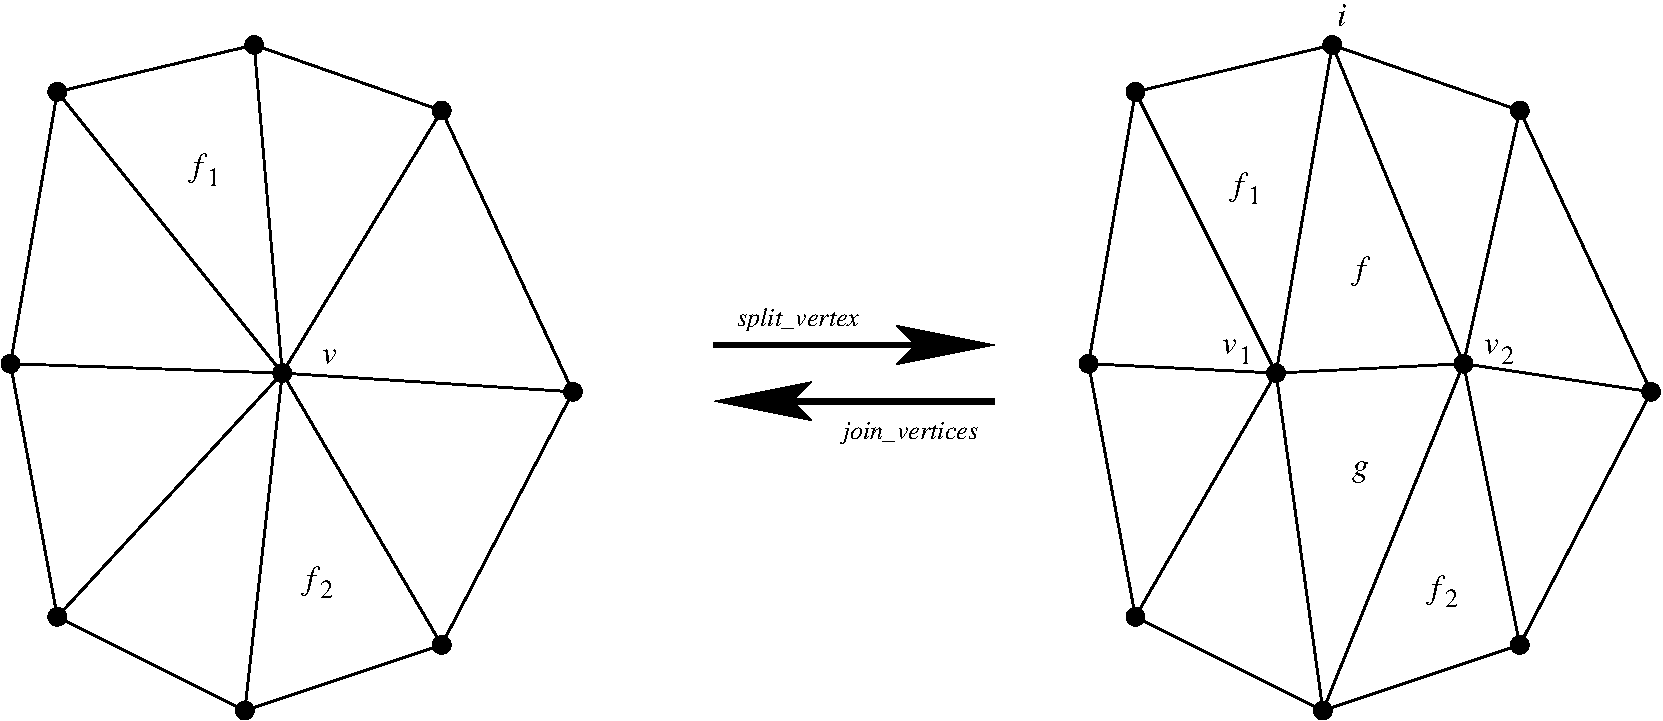
\includegraphics[width=0.95\textwidth]
{Segment_Delaunay_graph_2_ref/sdg-join_split}
\end{center}
\end{ccTexOnly}
\begin{ccHtmlOnly}
<center>
<img border=0 src="./sdg-join_split.gif" align=center
alt="The join and split operations''
title="The join and split operations">
</center>
\end{ccHtmlOnly}
\begin{ccHtmlOnly}
<br><font size=-1>
\end{ccHtmlOnly}
\caption{The join and split operations. Left to right:
The vertex \ccc{v} is split into $v_1$ and $v_2$. The faces $f$ and
$g$ are inserted after $f_1$ and $f_2$, respectively, in the
counter-clockwise sense. The vertices $v_1$, $v_2$ and the faces $f$
and $g$ are returned as a \ccc{boost} \ccc{tuple} in that order.
Right to left: The edge \ccc{(f,i)} is collapsed, and thus the
vertices $v_1$ and $v_2$ are joined. The vertex \ccc{v} is
returned.}
\begin{ccHtmlOnly}
</font>
\end{ccHtmlOnly}
\end{figure}



We only describe the additional requirements with respect to the
\ccc{ApolloniusGraphDataStructure_2} concept.

\ccRefines
\ccc{ApolloniusGraphDataStructure_2}

\ccHeading{Modification}
\ccThree{Vertex_handle}{sdgds.join_vertices(Face_handle v, int i)+}{}
%
\ccMethod{Vertex_handle join_vertices(Face_handle f, int i);}{Joins
  the vertices that are endpoints of the edge \ccc{(f,i)}. It returns
  a vertex handle to common vertex.}
\ccGlue
\ccMethod{boost::tuples::tuple<Vertex_handle, Vertex_handle, Face_handle,
Face_handle>
  split_vertex(Vertex_handle v, Face_handle f1, Face_handle
  f2);}{Splits the vertex \ccc{v} into two vertices \ccc{v1} and
  \ccc{v2}. The common faces \ccc{f} and \ccc{g} of \ccc{v1} and
  \ccc{v2} are created after (in the counter-clockwise sense) the
  faces \ccc{f1} and \ccc{f2}. The 4-tuple \ccc{(v1,v2,f,g)} is
  returned (see Fig. \ref{fig-sdgds-split-join}).}

\ccHasModels
\ccc{CGAL::Triangulation_data_structure_2<Vb,Fb>}

\ccSeeAlso
\ccc{TriangulationDataStructure_2}\\
\ccc{ApolloniusGraphDataStructure_2}\\
\ccc{SegmentDelaunayGraphVertexBase_2}\\
\ccc{TriangulationFaceBase_2}

\end{ccRefConcept}

% +------------------------------------------------------------------------+
%%RefPage: end of main body, begin of footer
% EOF
% +------------------------------------------------------------------------+

%% Copyright (c) 2003,2004,2005  INRIA Sophia-Antipolis (France) and
%% Notre Dame University (U.S.A.).  All rights reserved.
%%
%% This file is part of CGAL (www.cgal.org); you may redistribute it under
%% the terms of the Q Public License version 1.0.
%% See the file LICENSE.QPL distributed with CGAL.
%%
%% Licensees holding a valid commercial license may use this file in
%% accordance with the commercial license agreement provided with the software.
%%
%% This file is provided AS IS with NO WARRANTY OF ANY KIND, INCLUDING THE
%% WARRANTY OF DESIGN, MERCHANTABILITY AND FITNESS FOR A PARTICULAR PURPOSE.
%%
%% $URL$
%% $Id$ $Date$
%% 
%%
%% Author(s)     : Menelaos Karavelas <mkaravel@cse.nd.edu>



\begin{ccRefConcept}{SegmentDelaunayGraphVertexBase_2}

%% \ccHtmlCrossLink{}     %% add further rules for cross referencing links
%% \ccHtmlIndexC[concept]{} %% add further index entries
\ccCreationVariable{vb}
\ccDefinition

The concept \ccc{SegmentDelaunayGraphVertexBase_2} describes the
requirements for the vertex base class of the
\ccc{SegmentDelaunayGraphDataStructure_2} concept. A vertex stores a
site of the segment Delaunay graph and provides access to one of its
incident faces through a \ccc{Face_handle}.

\ccRefines
\ccc{DefaultConstructible}\\
\ccc{CopyConstructible}\\
\ccc{Assignable}

\ccTypes
%\ccTwo{SegmentDelaunayGraphVertexBase_2::Point_container+}{}
\ccThree{typedef typename Point_container::iterator+}{Point_handle+}{}
\ccThreeToTwo
\ccNestedType{Geom_traits}{A type for the geometric traits that defines
the site. \ccPrecond{The type \ccc{Geom_traits} must
define the type \ccc{Site_2}.}}
%
\ccGlue
\ccNestedType{Site_2}{A type for the site. This type must coincide
  with the type \ccc{Geom_traits::Site_2}.}
%
\ccGlue
\ccNestedType{Storage_site_tag}{A type that indicates what kind of
  storage type to use. \ccc{Storage_site_tag} must either be
    \ccc{CGAL::Tag_true} or \ccc{CGAL::Tag_false}.}
%
\ccGlue
\ccNestedType{Storage_site_2}{A type for the internal representation
  of sites. This type must satisfy the requirements of the concept
\ccc{SegmentDelaunayGraphStorageSite_2}.}
%
\ccGlue
\ccNestedType{Data_structure}{A type for the
  underlying data structure, to which the vertex belongs to.}
%
\ccGlue
\ccNestedType{Vertex_handle}{A type for the vertex handle of the
  segment Delaunay graph data structure.}
%
\ccGlue
\ccNestedType{Face_handle}{A type for the face handle of the
  segment Delaunay graph data structure.}
%

\ccCreation
\ccCreationVariable{v}  %% choose variable name

\ccTwo{SegmentDelaunayGraphVertexBase_2 v(Storage_site_2 ss);++}{}
%
%\ccConstructor{SegmentDelaunayGraphVertexBase_2();}{Default constructor.}
%\ccGlue

In addition to the default and copy constructors and following
constructors are required:

\ccConstructor{SegmentDelaunayGraphVertexBase_2(Storage_site_2 ss);}
{Constructs a vertex associated with the site represented by the
  storage site \ccc{ss}.}
\ccGlue
\ccConstructor{SegmentDelaunayGraphVertexBase_2(Storage_site_2 ss,
  Face_handle f);}{Constructs a vertex associated with
  the site represented by the storage site \ccc{ss},
  and pointing to the face associated with the face handle \ccc{f}.}





\ccAccessFunctions
\ccThree{Storage_site_2}{v.storage_site()+}{}
%
\ccMethod{Storage_site_2 storage_site();}
{Returns  the storage site representing the site.}
\ccGlue
\ccMethod{Site_2 site();}
{Returns  the site.}
\ccGlue
\ccMethod{Face_handle face();}{Returns a handle to an incident face.}



\ccHeading{Setting}
\ccThree{void}{v.set_site(Storage_site_2 ss)+}{}
\ccMethod{void set_site(Storage_site_2 ss);}
{Sets the storage site.}
\ccGlue
\ccMethod{void set_face(Face_handle f);}{Sets the incident face.}

\ccThree{bool}{v.is_valid(bool verbose, int level)+}{}
\ccHeading{Checking}
\ccMethod{bool is_valid(bool verbose, int level) const;}
{Performs any required tests on a vertex.}


\ccHasModels

\ccc{CGAL::Segment_Delaunay_graph_vertex_base_2<Gt>}.


\ccSeeAlso

\ccc{SegmentDelaunayGraphDataStructure_2}\\
\ccc{SegmentDelaunayGraphTraits_2}\\
\ccc{SegmentDelaunayGraphSite_2}\\
\ccc{SegmentDelaunayGraphStorageSite_2}\\
\ccc{CGAL::Segment_Delaunay_graph_vertex_base_2<Gt>}\\
\ccc{CGAL::Segment_Delaunay_graph_site_2<K>}\\
\ccc{CGAL::Segment_Delaunay_graph_storage_site_2<Gt,SSTag>}\\
\ccc{CGAL::Triangulation_data_structure_2<Vb,Fb>}

\end{ccRefConcept}

% +------------------------------------------------------------------------+
%%RefPage: end of main body, begin of footer
% EOF
% +------------------------------------------------------------------------+

%% Copyright (c) 2003,2004,2005  INRIA Sophia-Antipolis (France) and
%% Notre Dame University (U.S.A.).  All rights reserved.
%%
%% This file is part of CGAL (www.cgal.org); you may redistribute it under
%% the terms of the Q Public License version 1.0.
%% See the file LICENSE.QPL distributed with CGAL.
%%
%% Licensees holding a valid commercial license may use this file in
%% accordance with the commercial license agreement provided with the software.
%%
%% This file is provided AS IS with NO WARRANTY OF ANY KIND, INCLUDING THE
%% WARRANTY OF DESIGN, MERCHANTABILITY AND FITNESS FOR A PARTICULAR PURPOSE.
%%
%% $Source$
%% $Revision$ $Date$
%% $Name$
%%
%% Author(s)     : Menelaos Karavelas <mkaravel@cse.nd.edu>


\begin{ccRefClass}{Segment_Delaunay_graph_vertex_base_2<Gt,SSTag>}

%% add template arg's if necessary

%% \ccHtmlCrossLink{}     %% add further rules for cross referencing links
%% \ccHtmlIndexC[class]{} %% add further index entries
\ccCreationVariable{vb}
\ccDefinition

The class \ccRefName\ provides a model for the
\ccc{SegmentDelaunayGraphVertexBase_2} concept which is the vertex
base required by the \ccc{SegmentDelaunayGraphDataStructure_2}
concept. The class \ccRefName\ has two template arguments, the first
being the geometric traits of the segment Delaunay graph and should be a
model of the concept \ccc{SegmentDelaunayGraphTraits_2}.
The second template argument indicates whether
or not to use the simple storage site that does not support
intersecting segments, or the full storage site, that supports
intersecting segments. The possible values are \ccc{CGAL::Tag_true}
and \ccc{CGAL::Tag_false}. \ccc{CGAL::Tag_true} indicates that the
full storage site is to be used, whereas \ccc{CGAL::Tag_false}
indicates that the simple storage site is to be used.


\ccInclude{CGAL/Segment_Delaunay_graph_vertex_base_2.h}

\ccIsModel
\ccc{SegmentDelaunayGraphVertexBase_2}

%% \ccCreation
%% \ccCreationVariable{vb}  %% choose variable name
%% \ccTwo{Segment_Delaunay_graph_vertex_base_2<Gt>
%% vb(Storage_site_2 ss);++}{}

%% \ccConstructor{Segment_Delaunay_graph_vertex_base_2(Storage_site_2 ss);}
%% {Constructs a vertex associated with the storage site \ccc{ss}.}
%% \ccGlue
%% \ccConstructor{Segment_Delaunay_graph_vertex_base_2(Storage_site_2 ss, Face_handle f);}
%%               {Constructs a vertex associated with
%%                 the storage site \ccc{ss},
%%                 and pointing to the face associated with the face
%%                 handle \ccc{f}.}



\ccSeeAlso
\ccc{SegmentDelaunayGraphVertexBase_2}\\
\ccc{SegmentDelaunayGraphDataStructure_2}\\
\ccc{SegmentDelaunayGraphTraits_2}\\
\ccc{CGAL::Triangulation_data_structure_2<Vb,Fb>}\\
\ccc{CGAL::Segment_Delaunay_graph_traits_2<K,MTag>}\\
\ccc{CGAL::Segment_Delaunay_graph_traits_without_intersections_2<K,MTag>}\\
\ccc{CGAL::Segment_Delaunay_graph_filtered_traits_2<CK,CM,EK,EM,FK,FM>}\\
\ccc{CGAL::Segment_Delaunay_graph_filtered_traits_without_intersections_2<CK,CM,EK,EM,FK,FM>}
\end{ccRefClass}

% +------------------------------------------------------------------------+
%%RefPage: end of main body, begin of footer
% EOF
% +------------------------------------------------------------------------+


%% Copyright (c) 2003,2004,2005  INRIA Sophia-Antipolis (France) and
%% Notre Dame University (U.S.A.).  All rights reserved.
%%
%% This file is part of CGAL (www.cgal.org); you may redistribute it under
%% the terms of the Q Public License version 1.0.
%% See the file LICENSE.QPL distributed with CGAL.
%%
%% Licensees holding a valid commercial license may use this file in
%% accordance with the commercial license agreement provided with the software.
%%
%% This file is provided AS IS with NO WARRANTY OF ANY KIND, INCLUDING THE
%% WARRANTY OF DESIGN, MERCHANTABILITY AND FITNESS FOR A PARTICULAR PURPOSE.
%%
%% $URL$
%% $Id$
%% 
%%
%% Author(s)     : Menelaos Karavelas <mkaravel@cse.nd.edu>




\begin{ccRefConcept}{SegmentDelaunayGraphTraits_2}

%% \ccHtmlCrossLink{}     %% add further rules for cross referencing links
%% \ccHtmlIndexC[concept]{} %% add further index entries
\ccDefinition

The concept \ccc{SegmentDelaunayGraphTraits_2} provides the traits
requirements for the \ccc{Segment_Delaunay_graph_2<Gt,DS>} and
\ccc{Segment_Delaunay_graph_hierarchy_2<Gt,STag,DS>} classes. In
particular, it provides a type \ccc{Site_2}, which must be a model of
the concept \ccc{SegmentDelaunayGraphSite_2}. It also provides
constructions for sites and several function object
types for the predicates.

\ccRefines
\ccc{DefaultConstructible}\\
\ccc{CopyConstructible}\\
\ccc{Assignable}

\ccTypes
\ccTwo{SegmentDelaunayGraphTraits_2::Arrangement_type+}{}
%
\ccNestedType{Intersections_tag}{Indicates or not whether the
  intersecting segments are to be supported. The tag must either be
  \ccc{CGAL::Tag_true} or \ccc{CGAL::Tag_false}.}
\ccNestedType{Site_2}{A type for a site of the segment Delaunay
  graph. Must be a model of the concept
  \ccc{SegmentDelaunayGraphSite_2}.}
\ccGlue
\ccNestedType{Point_2}{A type for a point.}
\ccGlue
\ccNestedType{Line_2}{A type for a line. Only required if the segment
  Delaunay graph is inserted in a stream.}
\ccGlue
\ccNestedType{Ray_2}{A type for a ray. Only required if the segment
  Delaunay graph is inserted in a stream.}
\ccGlue
\ccNestedType{Segment_2}{A type for a segment. Only required if 
  if the segment Delaunay graph is inserted in a stream.}
\ccGlue
\ccNestedType{FT}{A type for the field number type of sites, points, etc..}
\ccGlue
\ccNestedType{RT}{A type for the ring number type of sites, points, etc.}
\ccGlue
\ccNestedType{Arrangement_type}{An enumeration type that indicates the
  type of the arrangement of two sites. The possible values are
  \ccc{DISJOINT}, \ccc{IDENTICAL}, \ccc{CROSSING},
  \ccc{TOUCHING_1}, \ccc{TOUCHING_2}, \ccc{TOUCHING_11},
  \ccc{TOUCHING_12}, \ccc{TOUCHING_21}, \ccc{TOUCHING_22},
  \ccc{OVERLAPPING_11}, \ccc{OVERLAPPING_12}, \ccc{OVERLAPPING_21},
  \ccc{OVERLAPPING_22}, \ccc{INTERIOR}, \ccc{INTERIOR_1},
  \ccc{INTERIOR_2}, \ccc{TOUCHING_11_INTERIOR_1},
  \ccc{TOUCHING_11_INTERIOR_2}, \ccc{TOUCHING_12_INTERIOR_1},
  \ccc{TOUCHING_12_INTERIOR_2}, \ccc{TOUCHING_21_INTERIOR_1},
  \ccc{TOUCHING_21_INTERIOR_2}, \ccc{TOUCHING_22_INTERIOR_1}, 
  \ccc{TOUCHING_22_INTERIOR_2}. A detailed description of the meaning
  of these values is shown the end of the reference manual for this
  concept. (\bf to be done)}
\ccGlue
\ccNestedType{Object_2}{A type representing different types of objects
  in two dimensions, namely: \ccc{Point_2}, \ccc{Site_2},
  \ccc{Line_2}, \ccc{Ray_2} and \ccc{Segment_2}.}
\ccGlue
\ccNestedType{Assign_2}
{Must provide \ccc{template <class T> bool operator() ( T& t,
    Object_2 o)} which assigns \ccc{o} to \ccc{t} if \ccc{o} was
  constructed from an object of type \ccc{T}. Returns 
  \ccc{true}, if the assignment was possible.}
\ccGlue
\ccNestedType{Construct_object_2}{Must provide \ccc{template <class T>
    Object_2 operator()( T t)} that constructs an object of type
  \ccc{Object_2} that contains \ccc{t} and returns it.}
\ccGlue
\ccNestedType{Construct_svd_vertex_2}{
  A constructor for a point of the segment Voronoi diagram equidistant
  from three sites. Must provide
  \ccc{Point_2 operator()(Site_2 s1, Site_2 s2, Site_2 s3)}, which
  constructs a point equidistant from the sites \ccc{s1}, \ccc{s2} and
  \ccc{s3}.
}
%
\ccTwo{SegmentDelaunayGraphTraits_2}{}
%
\ccGlue
\ccNestedType{Compare_x_2}{A predicate object type. Must
provide \ccc{Comparison_result operator()(Site_2 s1,
Site_2 s2)}, which compares the $x$-coordinates of the points
represented by the sites \ccc{s1} and \ccc{s2}.
\ccPrecond{\ccc{s1} and \ccc{s2} must be points.}}
%
\ccGlue
\ccNestedType{Compare_y_2}{A predicate object type. Must
provide \ccc{Comparison_result operator()(Site_2 s1,
Site_2 s2)}, which compares the $y$-coordinates of the points
represented by the sites \ccc{s1} and \ccc{s2}.
\ccPrecond{\ccc{s1} and \ccc{s2} must be points.}}
%
\ccGlue
\ccNestedType{Orientation_2}{A predicate object type. Must
provide \ccc{Orientation operator()(Site_2 s1,
Site_2 s2, Site_2 s3)}, which performs the
usual orientation test for three points.
\ccc{s1}, \ccc{s2} and \ccc{s3}.
\ccPrecond{the sites \ccc{s1}, \ccc{s2} and \ccc{s3} must be points.}}
%
\ccGlue
\ccNestedType{Equal_2}{A predicate object type. Must provide
  \ccc{bool operator()(Site_2 s1, Site_2 s2)}, which determines is the
  points represented by the sites \ccc{s1} and \ccc{s2} are identical.
  \ccPrecond{\ccc{s1} and \ccc{s2} must be points.}}
%
\ccGlue
\ccNestedType{Are_parallel_2}{A predicate object type. Must provide
  \ccc{bool operator()(Site_2 s1, Site_2 s2)}, which determines is the
  segments represented by the sites \ccc{s1} and \ccc{s2} are
  parallel.
  \ccPrecond{\ccc{s1} and \ccc{s2} must be segments.}}
%
\ccGlue
\ccNestedType{Oriented_side_of_bisector_2}{A predicate object type.
Must provide \ccc{Oriented_side operator()(Site_2 s1,
Site_2 s2, Point_2 p)}, which returns
the oriented side of the bisector of \ccc{s1} and \ccc{s2} that
contains \ccc{p}. Returns \ccc{ON_POSITIVE_SIDE} if \ccc{p} lies in
the half-space of \ccc{s1} (i.e., \ccc{p} is closer to \ccc{s1} than
\ccc{s2}); returns \ccc{ON_NEGATIVE_SIDE} if \ccc{p} lies in the
half-space of \ccc{s2}; returns \ccc{ON_ORIENTED_BOUNDARY} if \ccc{p}
lies on the bisector of \ccc{s1} and \ccc{s2}.}
%
\ccGlue
\ccNestedType{Vertex_conflict_2}{A predicate object type.
Must provide \ccc{Sign operator()(Site_2 s1, Site_2
s2, Site_2 s3, Site_2 q)}, which
returns the sign of the distance of \ccc{q} from the Voronoi circle
of \ccc{s1}, \ccc{s2}, \ccc{s3} (the Voronoi circle of three sites
\ccc{s1}, \ccc{s2}, \ccc{s3} is a circle co-tangent to all three
sites, that touches them in that order as we walk on its circumference
in the counter-clockwise sense).
\ccPrecond{the Voronoi circle of \ccc{s1}, \ccc{s2},
\ccc{s3} must exist.}\\
Must also provide \ccc{Sign operator()(Site_2 s1,
Site_2 s2, Site_2 q)}, which returns the sign of the distance of
\ccc{q} from the bitangent line of \ccc{s1}, \ccc{s2} (a degenerate
Voronoi circle, with its center at infinity).}
%
\ccGlue
\ccNestedType{Finite_edge_interior_conflict_2}{A predicate object
type. Must provide \ccc{bool operator()(Site_2 s1,
Site_2 s2, Site_2 s3, Site_2 s4,
Site_2 q, Sign sgn)}. The sites \ccc{s1}, \ccc{s2},
\ccc{s3} and \ccc{s4} define a Voronoi edge that lies on the
bisector of \ccc{s1} and \ccc{s2} and has as endpoints the Voronoi
vertices defined by the triplets \ccc{s1}, \ccc{s2}, \ccc{s3} and
\ccc{s1}, \ccc{s4} and \ccc{s2}. The sign \ccc{sgn} is the common sign
of the distance of the site \ccc{q} from the Voronoi circle of the
triplets \ccc{s1}, \ccc{s2}, \ccc{s3} and \ccc{s1}, \ccc{s4} and
\ccc{s2}. In case that \ccc{sgn} is equal to \ccc{NEGATIVE}, the
predicate returns \ccc{true} if and only if the entire Voronoi edge is
in conflict with \ccc{q}. If \ccc{sgn} is equal to \ccc{POSITIVE} or
\ccc{ZERO}, the predicate returns \ccc{false} if and only if \ccc{q}
is not in conflict with the Voronoi edge.
\ccPrecond{the Voronoi vertices of \ccc{s1}, \ccc{s2},
\ccc{s3}, and \ccc{s1}, \ccc{s4}, \ccc{s2} must exist.}\\
%
Must also provide \ccc{bool operator()(Site_2 s1,
Site_2 s2, Site_2 s3, Site_2 q, Sign sgn)}. The
sites \ccc{s1}, \ccc{s2}, \ccc{s3} and the site at infinity
$s_\infty$ define a Voronoi edge that lies on the bisector of
\ccc{s1} and \ccc{s2} and has as endpoints the Voronoi vertices
$v_{123}$ and $v_{1\infty{2}}$ defined by the triplets \ccc{s1},
\ccc{s2}, \ccc{s3} and \ccc{s1}, $s_\infty$ and \ccc{s2} (the second
vertex is actually at infinity). The sign \ccc{sgn} is the common sign
of the distance of the site \ccc{q} from the two Voronoi circles
centered at the Voronoi vertices $v_{123}$ and $v_{1\infty{2}}$.
In case that \ccc{sgn} is \ccc{NEGATIVE}, the predicate
returns \ccc{true} if and only if the entire Voronoi edge is in
conflict with \ccc{q}. If \ccc{sgn} is \ccc{POSITIVE} or \ccc{ZERO},
the predicate returns \ccc{false} if and only if \ccc{q} is not in
conflict with the Voronoi edge.
\ccPrecond{the Voronoi vertex $v_{123}$ of \ccc{s1}, \ccc{s2},
\ccc{s3} must exist.}\\
%
Must finally provide \ccc{bool operator()(Site_2 s1,
Site_2 s2, Site_2 q, Sign sgn)}. The
sites \ccc{s1}, \ccc{s2} and the site at infinity
$s_\infty$ define a Voronoi edge that lies on the bisector of
$v_{12\infty}$ and $v_{1\infty{}2}$
\ccc{s1} and \ccc{s2} and has as endpoints the Voronoi vertices
defined by the triplets \ccc{s1}, \ccc{s2}, $s_\infty$ and \ccc{s1},
$s_\infty$ and \ccc{s2} (both vertices are actually at
infinity). The sign \ccc{sgn} denotes the common sign of the distance
of the site \ccc{q} from the Voronoi circles centered at
$v_{12\infty}$ and $v_{1\infty{}2}$.
If \ccc{sgn} is \ccc{NEGATIVE}, the predicate
returns \ccc{true} if and only if the entire Voronoi edge is in
conflict with \ccc{q}. If \ccc{POSITIVE} or \ccc{ZERO} is \ccc{false},
the predicate returns \ccc{false} if and only if \ccc{q} is not in
conflict with the Voronoi edge.}
%
\ccGlue
\ccNestedType{Infinite_edge_interior_conflict_2}{A predicate
object type. Must provide \ccc{bool operator()(Site_2 s1,
Site_2 s2, Site_2 s3, Site_2 q, Sign sgn)}. The
sites $s_\infty$, \ccc{s1}, \ccc{s2} and \ccc{s3} define a
Voronoi edge that lies on the bisector of $s_\infty$ and \ccc{s1}
and has as endpoints the Voronoi vertices $v_{\infty{}12}$ and
$v_{\infty{}31}$ defined by the triplets
$s_\infty$, \ccc{s1}, \ccc{s2} and $s_\infty$, \ccc{s3} and
\ccc{s1}. The sign \ccc{sgn} is the common sign of the distances of
\ccc{q} from the Voronoi circles centered at the the vertices
$v_{\infty{}12}$ and $v_{\infty{}31}$. If \ccc{sgn} is \ccc{NEGATIVE},
the predicate returns \ccc{true} if and only if the entire Voronoi
edge is in conflict with \ccc{q}. If \ccc{sgn} is \ccc{POSITIVE} or
\ccc{ZERO}, the predicate returns \ccc{false} if and only if \ccc{q}
is not in conflict with the Voronoi edge.}
%
\ccGlue
\ccNestedType{Oriented_side_2}{A predicate object type. Must provide
  \ccc{Oriented_side operator()(Site_1 s1, Site_2 s2, Site_2 s3, Site_2
    s, Site_2 p)}. Determines the oriented side of the line $\ell$
  that contains the point site \ccc{p}, where $\ell$ is the line
  that passes through the Voronoi vertex of the sites \ccc{s1},
  \ccc{s2}, \ccc{s3} and is perpendicular to the segment site \ccc{s}.
  \ccPrecond{\ccc{s} must be a segment and \ccc{p} must be a point.}}
%
\ccNestedType{Arrangement_type_2}{A predicate object type. Must
  provide \ccc{Arrangement_type operator()(Site_2 s1, Site_2 s2)} that
  returns the type of the arrangement of the two sites \ccc{s1} and
  \ccc{s2}.}
%
 

\ccCreationVariable{gt}  %% choose variable name

%% \ccCreation

%% \ccThree{SegmentDelaunayGraphTraits_2}{ traits = other}{}
%% \ccThreeToTwo
%% %
%% \ccConstructor{ SegmentDelaunayGraphTraits_2(); }{Default constructor.}
%% \ccGlue
%% \ccConstructor{SegmentDelaunayGraphTraits_2(SegmentDelaunayGraphTraits_2
%% other);}{Copy constructor.}
%% \ccGlue
%% \ccMethod{SegmentDelaunayGraphTraits_2
%%   operator=(SegmentDelaunayGraphTraits_2 other);}
%% {Assignment operator.}



\ccHeading{Access to predicate objects}
%
\ccThree{Infinite_edge_interior_conflict_2}
{gt.infinite_edge_interior_conflict_2_object();}{}
%
\ccMethod{Compare_x_2 compare_x_2_object();}{}
\ccGlue
\ccMethod{Compare_y_2 compare_y_2_object();}{}
\ccGlue
\ccMethod{Orientation_2 orientation_2_object();}{}
\ccGlue
\ccMethod{Equal_2 equal_2_object();}{}
\ccGlue
\ccMethod{Are_parallel_2 are_parallel_2_object();}{}
\ccGlue
\ccMethod{Oriented_side_of_bisector_2
oriented_side_of_bisector_test_2_object();}{}
\ccGlue
\ccMethod{Vertex_conflict_2 vertex_conflict_2_object();}{}
\ccGlue
\ccMethod{Finite_edge_interior_conflict_2
        finite_edge_interior_conflict_2_object();}{}
\ccGlue
\ccMethod{Infinite_edge_interior_conflict_2
        infinite_edge_interior_conflict_2_object();}{}
\ccGlue
\ccMethod{Oriented_side_2 oriented_side_2_object();}{}
\ccGlue
\ccMethod{Arrangement_type_2 arrangement_type_2_object();}{}
%\ccGlue
%\ccMethod{Is_degenerate_edge_2 is_degenerate_edge_2_object();}{}




\ccHeading{Access to contructor objects}
%
\ccMethod{Construct_object_2
construct_object_2_object();}{} 
%
\ccGlue
\ccMethod{Construct_svd_vertex_2
construct_svd_vertex_2_object();}{} 
%




\ccHeading{Access to other objects}
%
\ccMethod{Assign_2 assign_2_object();}{} 


\ccHasModels

\ccc{CGAL::Segment_Delaunay_graph_traits_2<K,MTag>}\\
\ccc{CGAL::Segment_Delaunay_graph_traits_without_intersections_2<K,MTag>}\\
\ccc{CGAL::Segment_Delaunay_graph_filtered_traits_2<CK,CM,EK,EM,FK,FM>}\\
\ccc{CGAL::Segment_Delaunay_graph_filtered_traits_without_intersections_2<CK,CM,EK,EM,FK,FM>}


\ccSeeAlso
\ccc{SegmentDelaunayGraphSite_2}\\
\ccc{CGAL::Segment_Delaunay_graph_2<Gt,DS>}\\
\ccc{CGAL::Segment_Delaunay_graph_hierarchy_2<Gt,STag,DS>}\\
\ccc{CGAL::Segment_Delaunay_graph_traits_2<K,MTag>}\\
\ccc{CGAL::Segment_Delaunay_graph_traits_without_intersections_2<K,MTag>}\\
\ccc{CGAL::Segment_Delaunay_graph_filtered_traits_2<CK,CM,EK,EM,FK,FM>}\\
\ccc{CGAL::Segment_Delaunay_graph_filtered_traits_without_intersections_2<CK,CM,EK,EM,FK,FM>}
\end{ccRefConcept}

% +------------------------------------------------------------------------+
%%RefPage: end of main body, begin of footer
% EOF
% +------------------------------------------------------------------------+


%% Copyright (c) 2003,2004,2005  INRIA Sophia-Antipolis (France).
%% All rights reserved.
%%
%% This file is part of CGAL (www.cgal.org); you may redistribute it under
%% the terms of the Q Public License version 1.0.
%% See the file LICENSE.QPL distributed with CGAL.
%%
%% Licensees holding a valid commercial license may use this file in
%% accordance with the commercial license agreement provided with the software.
%%
%% This file is provided AS IS with NO WARRANTY OF ANY KIND, INCLUDING THE
%% WARRANTY OF DESIGN, MERCHANTABILITY AND FITNESS FOR A PARTICULAR PURPOSE.
%%
%% $URL$
%% $Id$
%% 
%%
%% Author(s)     : Menelaos Karavelas <mkaravel@iacm.forth.gr>



\begin{ccRefClass}{Segment_Delaunay_graph_traits_2<K,MTag>}
%% add template arg's if necessary

%% \ccHtmlCrossLink{}     %% add further rules for cross referencing links
%% \ccHtmlIndexC[class]{} %% add further index entries

\ccDefinition
  
The class \ccRefName\ provides a model for the
\ccc{SegmentDelaunayGraphTraits_2} concept.
This class has two template parameters. The first template parameter
must be a model of the \ccc{Kernel} concept. The second template
parameter corresponds to how predicates are evaluated. There are two
possible values for \ccc{MTag}, namely \ccc{CGAL::Field_with_sqrt_tag} and
\ccc{CGAL::Field_tag}. The first one must be used when the number type
used in the representation supports the exact evaluation of signs of
expressions involving all four basic operations and square roots,
whereas the second one requires the exact evaluation of signs of
field-type expressions, i.e., expressions involving additions,
subtractions, multiplications and divisions. The default value for
\ccc{MTag} is \ccc{CGAL::Field_tag}.
%
The way the predicates are evaluated is discussed in
\cite{b-ecvdl-96} and \cite{cgal:k-reisv-04} (the geometric filtering
part).


\ccInclude{CGAL/Segment_Delaunay_graph_traits_2.h}

\ccIsModel
\ccc{SegmentDelaunayGraphTraits_2}

\ccTypes
\ccThree{typedef CGAL::Tag_true}{Intersections_tag;}{}
\ccTypedef{typedef CGAL::Tag_true Intersections_tag;}{}

The \ccRefName\ class introduces a few additional types with respect
to the \ccc{SegmentDelaunayGraphTraits_2} concept. These are:

\ccTypedef{typedef K Kernel;}{A typedef for the template parameter
  \ccc{K}.}
\ccGlue
\ccTypedef{typedef MTag Method_tag;}{A typedef for the template
  parameter \ccc{MTag}.}

\ccCreationVariable{traits}

\ccSeeAlso
\ccc{Kernel}\\
\ccc{SegmentDelaunayGraphTraits_2} \\
\ccc{CGAL::Field_tag}\\
\ccc{CGAL::Field_with_sqrt_tag}\\
\ccc{CGAL::Segment_Delaunay_graph_2<Gt,DS>}\\
\ccc{CGAL::Segment_Delaunay_graph_hierarchy_2<Gt,STag,DS>}\\
\ccc{CGAL::Segment_Delaunay_graph_traits_without_intersections_2<K,MTag>}\\
\ccc{CGAL::Segment_Delaunay_graph_filtered_traits_2<CK,CM,EK,EM,FK,FM>}\\
\ccc{CGAL::Segment_Delaunay_graph_filtered_traits_without_intersections_2<CK,CM,EK,EM,FK,FM>}

\end{ccRefClass}

% +------------------------------------------------------------------------+
%%RefPage: end of main body, begin of footer
% EOF
% +------------------------------------------------------------------------+


%% Copyright (c) 2003,2004,2005  INRIA Sophia-Antipolis (France) and
%% Notre Dame University (U.S.A.).  All rights reserved.
%%
%% This file is part of CGAL (www.cgal.org); you may redistribute it under
%% the terms of the Q Public License version 1.0.
%% See the file LICENSE.QPL distributed with CGAL.
%%
%% Licensees holding a valid commercial license may use this file in
%% accordance with the commercial license agreement provided with the software.
%%
%% This file is provided AS IS with NO WARRANTY OF ANY KIND, INCLUDING THE
%% WARRANTY OF DESIGN, MERCHANTABILITY AND FITNESS FOR A PARTICULAR PURPOSE.
%%
%% $URL$
%% $Id$
%% 
%%
%% Author(s)     : Menelaos Karavelas <mkaravel@cse.nd.edu>



\begin{ccRefClass}{Segment_Delaunay_graph_traits_without_intersections_2<K,MTag>}
%% add template arg's if necessary

%% \ccHtmlCrossLink{}     %% add further rules for cross referencing links
%% \ccHtmlIndexC[class]{} %% add further index entries

\ccDefinition
  
The class \ccRefName\ provides a model for the
\ccc{SegmentDelaunayGraphTraits_2} concept.
This class has two template parameters. 
The first template parameter must be a model of the \ccc{Kernel}
concept. The second template parameter corresponds to how predicates
are evaluated. There are two possible values for \ccc{MTag}, namely
\ccc{CGAL::Field_with_sqrt_tag} and \ccc{CGAL::Euclidean_ring_tag}. The first one
must be used when the number type used in the representation supports
the exact evaluation of signs of expressions involving all four basic
operations and square roots, whereas the second one requires the exact
evaluation of signs of ring-type expressions, i.e., expressions
involving only additions, subtractions and multiplications. The
default value for \ccc{MTag} is \ccc{CGAL::Euclidean_ring_tag}.
%
The way the predicates are evaluated is discussed in
\cite{b-ecvdl-96} and \cite{cgal:k-reisv-04} (the geometric filtering
part).


\ccInclude{CGAL/Segment_Delaunay_graph_traits_2.h}

\ccIsModel
\ccc{SegmentDelaunayGraphTraits_2}

\ccTypes
\ccThree{typedef CGAL::Tag_false}{Intersections_tag;}{}
\ccTypedef{typedef CGAL::Tag_false Intersections_tag;}{}

The \ccRefName\ class introduces a few additional types with respect
to the \ccc{SegmentDelaunayGraphTraits_2} concept. These are:

\ccTypedef{typedef K Kernel;}{A typedef for the template parameter
  \ccc{K}.}
\ccGlue
\ccTypedef{typedef MTag Method_tag;}{A typedef for the template
  parameter \ccc{MTag}.}

\ccCreationVariable{traits}

\ccSeeAlso
\ccc{Kernel}\\
\ccc{SegmentDelaunayGraphTraits_2} \\
\ccc{CGAL::Euclidean_ring_tag}\\
\ccc{CGAL::Field_with_sqrt_tag}\\
\ccc{CGAL::Segment_Delaunay_graph_2<Gt,DS>}\\
\ccc{CGAL::Segment_Delaunay_graph_hierarchy_2<Gt,STag,DS>}\\
\ccc{CGAL::Segment_Delaunay_graph_traits_2<K,MTag>}\\
\ccc{CGAL::Segment_Delaunay_graph_filtered_traits_2<CK,CM,EK,EM,FK,FM>}\\
\ccc{CGAL::Segment_Delaunay_graph_filtered_traits_without_intersections_2<CK,CM,EK,EM,FK,FM>}

\end{ccRefClass}

% +------------------------------------------------------------------------+
%%RefPage: end of main body, begin of footer
% EOF
% +------------------------------------------------------------------------+


%% Copyright (c) 2003,2004,2005  INRIA Sophia-Antipolis (France) and
%% Notre Dame University (U.S.A.).  All rights reserved.
%%
%% This file is part of CGAL (www.cgal.org); you may redistribute it under
%% the terms of the Q Public License version 1.0.
%% See the file LICENSE.QPL distributed with CGAL.
%%
%% Licensees holding a valid commercial license may use this file in
%% accordance with the commercial license agreement provided with the software.
%%
%% This file is provided AS IS with NO WARRANTY OF ANY KIND, INCLUDING THE
%% WARRANTY OF DESIGN, MERCHANTABILITY AND FITNESS FOR A PARTICULAR PURPOSE.
%%
%% $URL$
%% $Id$
%% 
%%
%% Author(s)     : Menelaos Karavelas <mkaravel@cse.nd.edu>



\begin{ccRefClass}
{Segment_Delaunay_graph_filtered_traits_2<CK,CM,EK,EM,FK,FM>}
%% add template arg's if necessary

%% \ccHtmlCrossLink{}     %% add further rules for cross referencing links
%% \ccHtmlIndexC[class]{} %% add further index entries

\ccDefinition
  
The class \ccRefName\ provides a model for the
\ccc{SegmentDelaunayGraphTraits_2} concept.

The class \ccRefName\ uses the filtering technique \cite{cgal:bbp-iayed-01}
to achieve traits for the \ccc{Segment_Delaunay_graph_2<Gt,DS>}
class with efficient and exact predicates given an exact
kernel \ccc{EK} and a filtering kernel \ccc{FK}. The geometric
constructions associated provided by this class are equivalent
to those provided by the traits class
\ccc{Segment_Delaunay_graph_traits_2<CK,CM>}, which means that
they may be inexact depending on the choice of the \ccc{CK} kernel.

This class has six template parameters. The first, third and fifth
template parameters must be a models of the \ccc{Kernel} concept. The
parameter \ccc{CK} is the construction kernel and it is the kernel
that will be used for constructions. The parameter \ccc{FK} is the
filtering kernel; this kernel will be used for performing the
arithmetic filtering for the predicates involved in the computation of
the segment Delaunay graph. Finally, the parameter \ccc{EK} is the
exact kernel; this kernel will be used for computing the predicates if
the filtering kernel fails to produce an answer.

The second, fourth and sixth template parameters correspond to how
predicates are evaluated. There are two predefined possible values for
these parameters, namely \ccc{CGAL::Field_with_sqrt_tag} and
\ccc{CGAL::Field_tag}. The first one must be used when the number type
used in the representation supports the exact evaluation of signs of
expressions involving all four basic operations and square roots,
whereas the second one requires that only field operations are
exact. Finally, in order to get exact constructions \ccc{CM}
must be set to \ccc{CGAL::Field_with_sqrt_tag} and the number type in
\ccc{CK} must support operations involing divisions and square roots
(as well as the other three basic operations of course).
%
The way the predicates are evaluated is discussed in
\cite{b-ecvdl-96} and \cite{cgal:k-reisv-04} (the geometric filtering
part).

The default values for the template parameters are as follows:
\ccc{CM = CGAL::Field_with_sqrt_tag} (it is assumed that
\ccc{CGAL::Cartesian<double>} or \ccc{CGAL::Simple_cartesian<double>}
will be the entry for the template parameter \ccc{CK}), 
\ccc{EM = CGAL::Field_tag},
\ccc{FK = CGAL::Simple_cartesian<CGAL::Interval_nt<false> >},
\ccc{FM = CGAL::Field_with_sqrt_tag}. If the \textsc{Gmp} package is
installed with \cgal, the template parameter \ccc{EK} has the default
value: \ccc{EK = CGAL::Simple_cartesian<CGAL::Gmpq>}, otherwise its
default value is
\ccc{EK = CGAL::Simple_cartesian<CGAL::Quotient<CGAL::MP_Float> >}.


\ccInclude{CGAL/Segment_Delaunay_graph_filtered_traits_2.h}

\ccIsModel
\ccc{SegmentDelaunayGraphTraits_2}\\
\ccc{DefaultConstructible}\\
\ccc{CopyConstructible}\\
\ccc{Assignable}

\ccTypes

\ccThree{typedef CGAL::Tag_true}{Intersections_tag;}{}
\ccTypedef{typedef CGAL::Tag_true Intersections_tag;}{}

In addition to the types required by the
\ccc{SegmentDelaunayGraphTraits_2} concept the class \ccRefName\
defines the following types:

\ccTypedef{typedef CK  Kernel;}{}
\ccGlue
\ccTypedef{typedef CK  Construction_kernel;}{}
\ccGlue
\ccTypedef{typedef FK  Filtering_kernel;}{}
\ccGlue
\ccTypedef{typedef EK  Exact_kernel;}{}
\ccGlue
\ccTypedef{typedef CM  Method_tag;}{}
\ccGlue
\ccTypedef{typedef CM  Construction_traits_method_tag;}{}
\ccGlue
\ccTypedef{typedef FM  Filtering_traits_method_tag;}{}
\ccGlue
\ccTypedef{typedef EM  Exact_traits_method_tag;}{}
\ccGlue
\ccNestedType{Construction_traits}{A type for the segment Delaunay
  graph traits, where the kernel is \ccc{CK}.}
\ccGlue
\ccNestedType{Filtering_traits}{A type for the segment Delaunay
  graph traits, where the kernel is \ccc{FK}.}
\ccGlue
\ccNestedType{Exact_traits}{A type for the segment Delaunay
  graph traits, where the kernel is \ccc{EK}.}



\ccSeeAlso
\ccc{Kernel}\\
\ccc{SegmentDelaunayGraphTraits_2} \\
\ccc{CGAL::Field_tag}\\
\ccc{CGAL::Field_with_sqrt_tag}\\
\ccc{CGAL::Segment_Delaunay_graph_2<Gt,DS>}\\
\ccc{CGAL::Segment_Delaunay_graph_hierarchy_2<Gt,STag,DS>}\\
\ccc{CGAL::Segment_Delaunay_graph_traits_2<K,MTag>}\\
\ccc{CGAL::Segment_Delaunay_graph_traits_without_intersections_2<K,MTag>}\\
\ccc{CGAL::Segment_Delaunay_graph_filtered_traits_without_intersections_2<CK,CM,EK,EM,FK,FM>}


\end{ccRefClass}

% +------------------------------------------------------------------------+
%%RefPage: end of main body, begin of footer
% EOF
% +------------------------------------------------------------------------+


%% Copyright (c) 2003,2004,2005  INRIA Sophia-Antipolis (France) and
%% Notre Dame University (U.S.A.).  All rights reserved.
%%
%% This file is part of CGAL (www.cgal.org); you may redistribute it under
%% the terms of the Q Public License version 1.0.
%% See the file LICENSE.QPL distributed with CGAL.
%%
%% Licensees holding a valid commercial license may use this file in
%% accordance with the commercial license agreement provided with the software.
%%
%% This file is provided AS IS with NO WARRANTY OF ANY KIND, INCLUDING THE
%% WARRANTY OF DESIGN, MERCHANTABILITY AND FITNESS FOR A PARTICULAR PURPOSE.
%%
%% $URL$
%% $Id$ $Date$
%% 
%%
%% Author(s)     : Menelaos Karavelas <mkaravel@cse.nd.edu>



\begin{ccRefClass}
{Segment_Delaunay_graph_filtered_traits_without_intersections_2<CK,CM,EK,EM,FK,FM>}
%% add template arg's if necessary

%% \ccHtmlCrossLink{}     %% add further rules for cross referencing links
%% \ccHtmlIndexC[class]{} %% add further index entries

\ccDefinition
  
The class \ccRefName\ provides a model for the
\ccc{SegmentDelaunayGraphTraits_2} concept.

The class \ccRefName\ uses the filtering technique \cite{cgal:bbp-iayed-01}
to achieve traits for the \ccc{Segment_Delaunay_graph_2<Gt,DS>}
class with efficient and exact predicates given an exact
kernel \ccc{EK} and a filtering kernel \ccc{FK}. The geometric
constructions associated provided by this class are equivalent
to those provided by the traits class
\ccc{Segment_Delaunay_graph_traits_without_intersections_2<CK,CM>},
which means that they may be inexact, depending on the choice of the
\ccc{CK} kernel.

This class has six template parameters. The first, third and fifth
template parameters must be a models of the \ccc{Kernel} concept. The
parameter \ccc{CK} is the construction kernel and it is the kernel
that will be used for constructions. The parameter \ccc{FK} is the
filtering kernel; this kernel will be used for performing the
arithmetic filtering for the predicates involved in the computation of
the segment Delaunay graph. Finally, the parameter \ccc{EK} is the
exact kernel; this kernel will be used for computing the predicates if
the filtering kernel fails to produce an answer.

The second, fourth and sixth template parameters
correspond to how predicates are evaluated. There are two predefined
possible values for these parameters, namely \ccc{CGAL::Sqrt_field_tag}
and \ccc{CGAL::Ring_tag}. The first one must be used when the number
type used in the representation supports the exact evaluation of signs
of expressions involving all four basic operations and square roots,
whereas the second requires the exact evaluation of signs of ring-type
expressions, i.e., expressions involving only additions, subtractions
and multiplications. Finally, in order to get exact constructions
\ccc{CM} must be set to \ccc{CGAL::Sqrt_field_tag} and the number type
in \ccc{CK} must support operations involing divisions and square
roots (as well as the other three basic operations of course).
%
The way the predicates are evaluated is discussed in
\cite{b-ecvdl-96} and \cite{cgal:k-reisv-04} (the geometric filtering
part).

The default values for the template parameters are as follows:
\ccc{CM = CGAL::Sqrt_field_tag} (it is assumed that
\ccc{CGAL::Cartesian<double>} or \ccc{CGAL::Simple_cartesian<double>}
will be the entry for the template parameter \ccc{CK}), 
\ccc{EM = CGAL::Ring_tag},
\ccc{FK = CGAL::Simple_cartesian<CGAL::Interval_nt<false> >},
\ccc{FM = CGAL::Sqrt_field_tag}. If the \textsc{Gmp} package is
installed with \cgal, the template parameter \ccc{EK} has the default
value: \ccc{EK = CGAL::Simple_cartesian<CGAL::Gmpq>}, otherwise its
default value is
\ccc{EK = CGAL::Simple_cartesian<CGAL::MP_Float>}.


\ccInclude{CGAL/Segment_Delaunay_graph_filtered_traits_2.h}

\ccIsModel
\ccc{SegmentDelaunayGraphTraits_2}\\
\ccc{DefaultConstructible}\\
\ccc{CopyConstructible}\\
\ccc{Assignable}

\ccTypes

\ccThree{typedef CGAL::Tag_false}{Intersections_tag;}{}
\ccTypedef{typedef CGAL::Tag_false Intersections_tag;}{}

In addition to the types required by the
\ccc{SegmentDelaunayGraphTraits_2} concept the class \ccRefName\
defines the following types:

\ccTypedef{typedef CK  Kernel;}{}
\ccGlue
\ccTypedef{typedef CK  Construction_kernel;}{}
\ccGlue
\ccTypedef{typedef FK  Filtering_kernel;}{}
\ccGlue
\ccTypedef{typedef EK  Exact_kernel;}{}
\ccGlue
\ccTypedef{typedef CM  Method_tag;}{}
\ccGlue
\ccTypedef{typedef CM  Construction_traits_method_tag;}{}
\ccGlue
\ccTypedef{typedef FM  Filtering_traits_method_tag;}{}
\ccGlue
\ccTypedef{typedef EM  Exact_traits_method_tag;}{}
\ccGlue
\ccNestedType{Construction_traits;}{A type for the segment Delaunay
  graph traits, where the kernel is \ccc{CK}.}
\ccGlue
\ccNestedType{Filtering_traits;}{A type for the segment Delaunay
  graph traits, where the kernel is \ccc{FK}.}
\ccGlue
\ccNestedType{Exact_traits;}{A type for the segment Delaunay
  graph traits, where the kernel is \ccc{EK}.}



\ccSeeAlso
\ccc{Kernel}\\
\ccc{SegmentDelaunayGraphTraits_2} \\
\ccc{CGAL::Ring_tag}\\
\ccc{CGAL::Sqrt_field_tag}\\
\ccc{CGAL::Segment_Delaunay_graph_2<Gt,DS>}\\
\ccc{CGAL::Segment_Delaunay_graph_hierarchy_2<Gt,STag,DS>}\\
\ccc{CGAL::Segment_Delaunay_graph_traits_2<K,MTag>}\\
\ccc{CGAL::Segment_Delaunay_graph_traits_without_intersections_2<K,MTag>}\\
\ccc{CGAL::Segment_Delaunay_graph_filtered_traits_2<CK,CM,EK,EM,FK,FM>}

\end{ccRefClass}

% +------------------------------------------------------------------------+
%%RefPage: end of main body, begin of footer
% EOF
% +------------------------------------------------------------------------+


%% Copyright (c) 2003,2004,2005  INRIA Sophia-Antipolis (France) and
%% Notre Dame University (U.S.A.).  All rights reserved.
%%
%% This file is part of CGAL (www.cgal.org); you may redistribute it under
%% the terms of the Q Public License version 1.0.
%% See the file LICENSE.QPL distributed with CGAL.
%%
%% Licensees holding a valid commercial license may use this file in
%% accordance with the commercial license agreement provided with the software.
%%
%% This file is provided AS IS with NO WARRANTY OF ANY KIND, INCLUDING THE
%% WARRANTY OF DESIGN, MERCHANTABILITY AND FITNESS FOR A PARTICULAR PURPOSE.
%%
%% $URL$
%% $Id$ $Date$
%% 
%%
%% Author(s)     : Menelaos Karavelas <mkaravel@cse.nd.edu>



\begin{ccRefClass}{Segment_Delaunay_graph_hierarchy_2<Gt,STag,DS>}
%% add template arg's if necessary

%% \ccHtmlCrossLink{}     %% add further rules for cross referencing links
%% \ccHtmlIndexC[class]{} %% add further index entries
\ccDefinition

We provide an alternative to the class
\ccc{Segment_Delaunay_graph_2<Gt,DS>} for the incremental
construction of the segment Delaunay graph. The \ccRefName\ class
maintains a hierarchy of Delaunay graphs. There are two possibilities
as to how this hierarchy is constructed.

In the first case the bottom-most level of the hierarchy contains the
full segment Delaunay graph. The upper levels of the hierarchy
contain only points that are either point sites or endpoints of
segment sites in the bottom-most Delaunay graph. 
A point that is in level $i$ (either as an individdual point or as the
endpoint of a segment), is inserted in level $i+1$ with probability
$1/\alpha$ where $\alpha>1$ is some constant.
In the second case the upper levels of the hierarchy contains not only
points but also segments. A site that is in level $i$, is in level
$i+1$ with probability $1/\beta$ where $\beta > 1$ is some constant.

The difference between the \ccc{Segment_Delaunay_graph_2<Gt,DS>}
class and the \ccRefName\ class (both versions of it) is on how the
nearest neighbor location is done. Given a point $p$ the location is
done as follows: at the top most level we find the nearest neighbor of
$p$ as in the \ccc{Segment_Delaunay_graph_2<Gt,DS>} class. At
every subsequent level $i$ we use the nearest neighbor found at level
$i+1$ to find the nearest neighbor at level $i$. This is a variant of
the corresponding hierarchy for points found in \cite{cgal:d-dh-02}. The
details are described in \cite{cgal:k-reisv-04}.

The class has three template parameters. The first and third
have essentially the same semantics as in the
\ccc{Segment_Delaunay_graph_2<Gt,DS>} class. The
first template parameter must be a model of the
\ccc{SegmentDelaunayGraphTraits_2} concept. The third template
parameter must be a model of the
\ccc{SegmentDelaunayGraphDataStructure_2} concept. However, the
vertex base class that is to be used in the segment Delaunay graph
data structure must be a model of the
\ccc{SegmentDelaunayGraphHierarchyVertexBase_2}
concept. The third template parameter defaults to
\ccc{Triangulation_data_structure_2<
Segment_Delaunay_graph_hierarchy_vertex_base_2< 
Segment_Delaunay_graph_vertex_base_2<Gt> >,
Triangulation_face_base_2<Gt> >}. The second template
parameter controls whether or not segments are added in the upper
levels of the hierarchy. It's possible values are \ccc{CGAL::Tag_true}
and \ccc{CGAL::Tag_false}. If it is set to \ccc{CGAL::Tag_true},
segments are also inserted in the upper levels of the hierarchy. The
value \ccc{CGAL::Tag_false} indicates that only points are to be
inserted in the upper levels of the hierarchy. The default value for
the second template parameter is \ccc{CGAL::Tag_false}.


The \ccRefName\ class derives publicly from the
\ccc{Segment_Delaunay_graph_2<Gt,DS>} class. The interface is
the same with its base class. In the sequel only additional types
and methods defined are documented.


\ccInclude{CGAL/Segment_Delaunay_graph_hierarchy_2.h}


\ccIsModel
\ccc{DefaultConstructible}\\
\ccc{CopyConstructible}\\
\ccc{Assignable}

\ccInheritsFrom
\ccc{CGAL::Segment_Delaunay_graph_2<Gt,DS>}


\ccTypes
\ccRefName\ introduces the following types in addition to those
introduced by its base class \ccc{Segment_Delaunay_graph_2<Gt,DS>}.

\ccThree{typedef CGAL::Segment_Delaunay_graph_2<Gt,DS>}{Base+}{}
\ccThreeToTwo
\ccTypedef{typedef STag Segments_in_hierarchy_tag;}{A type for the
  \ccc{STag} template parameter.}
\ccGlue
\ccTypedef{typedef CGAL::Segment_Delaunay_graph_2<Gt,DS> Base;}
          {A type for the base class.}

\ccCreation
\ccCreationVariable{sdgh}
%
\ccThree{Segment_Delaunay_graph_hierarchy_2<Gt,STag,DS>}
{sdgh(Gt gt=Gt());}{}
\ccThreeToTwo
\ccTwo{Segment_Delaunay_graph_hierarchy}{}

In addition to the default and copy constructors, the following
constructors are defined:

\ccConstructor{Segment_Delaunay_graph_hierarchy_2(Gt
gt=Gt())}{Creates a hierarchy of segment Delaunay graphs using
  \ccc{gt} as geometric traits.}
%
\ccGlue
\ccConstructor{template< class Input_iterator >
Segment_Delaunay_graph_hierarchy_2<Gt,STag,DS>(Input_iterator
first, Input_iterator beyond, Gt gt=Gt())}
{Creates a segment Delaunay graph hierarchy using 
\ccc{gt} as geometric traits and inserts all sites in the
range [\ccc{first}, \ccc{beyond}). \ccc{Input_iterator} must be a
  model of \ccc{InputIterator}. The value type of \ccc{Input_iterator}
  must be either \ccc{Point_2} or \ccc{Site_2}.}
%
%% \ccGlue
%% \ccConstructor{Segment_Delaunay_graph_hierarchy_2<Gt,STag,DS>
%% (Segment_Delaunay_graph_hierarchy_2<Gt,STag,DS> other)}
%% {Copy constructor. All faces, vertices and inter-level pointers
%% are duplicated. After the construction, \ccVar\ and \ccc{other} refer
%% to two different hierarchies: if \ccc{other} is modified, \ccVar\ is
%% not.}
%% %
%% \ccThree{Segment_Delaunay_graph_hierarchy<Gt,STag,PC,DS>++}{svdh = other;}{}
%% \ccThreeToTwo
%% \ccGlue
%% \ccMethod{Segment_Delaunay_graph_hierarchy_2<Gt,STag,DS>
%% operator=(Segment_Delaunay_graph_hierarchy_2<Gt,STag,DS>
%% other);}{Assignment. All faces, vertices and inter-level pointers
%% are duplicated. After the construction, \ccVar\ and \ccc{other} refer
%% to two different hierarchies: if \ccc{other} is modified, \ccVar\ is
%% not.}

\ccHeading{I/O}
\ccThree{std::ostream&}{std::ostream& os ++ sdgh+}{}
\ccThreeToTwo
%
\ccFunction{std::ostream& operator<<(std::ostream& os,
  Segment_Delaunay_graph_hierarchy_2<Gt,STag,DS> svdh);}
{Writes the current state of the segment Delaunay graph hierarchy to
  an output stream. In particular, all sites in the diagram are
  written to the stream (represented through appropriate input sites),
  as well as the underlying combinatorial hierarchical data structure.}
\ccGlue
\ccFunction{std::istream& operator>>(std::istream& is,
  Segment_Delaunay_graph_hierarchy_2<Gt,STag,DS> svdh);}
{Reads the state of the segment Delaunay graph hierarchy from an
  input stream.}


\ccSeeAlso
\ccc{SegmentDelaunayGraphDataStructure_2}\\
\ccc{SegmentDelaunayGraphTraits_2}\\
\ccc{SegmentDelaunayGraphHierarchyVertexBase_2}\\
\ccc{CGAL::Segment_Delaunay_graph_2<Gt,DS>}\\
\ccc{CGAL::Triangulation_data_structure_2<Vb,Fb>}\\
\ccc{CGAL::Segment_Delaunay_graph_traits_2<K,MTag>}\\
\ccc{CGAL::Segment_Delaunay_graph_traits_without_intersections_2<K,MTag>}\\
\ccc{CGAL::Segment_Delaunay_graph_filtered_traits_2<CK,CM,EK,EM,FK,FM>}\\
\ccc{CGAL::Segment_Delaunay_graph_filtered_traits_without_intersections_2<CK,CM,EK,EM,FK,FM>}\\
\ccc{CGAL::Segment_Delaunay_graph_hierarchy_vertex_base_2<Vbb>}

\end{ccRefClass}

% +------------------------------------------------------------------------+
%%RefPage: end of main body, begin of footer
% EOF
% +------------------------------------------------------------------------+

%% Copyright (c) 2003,2004,2005  INRIA Sophia-Antipolis (France) and
%% Notre Dame University (U.S.A.).  All rights reserved.
%%
%% This file is part of CGAL (www.cgal.org); you may redistribute it under
%% the terms of the Q Public License version 1.0.
%% See the file LICENSE.QPL distributed with CGAL.
%%
%% Licensees holding a valid commercial license may use this file in
%% accordance with the commercial license agreement provided with the software.
%%
%% This file is provided AS IS with NO WARRANTY OF ANY KIND, INCLUDING THE
%% WARRANTY OF DESIGN, MERCHANTABILITY AND FITNESS FOR A PARTICULAR PURPOSE.
%%
%% $Source$
%% $Revision$ $Date$
%% $Name$
%%
%% Author(s)     : Menelaos Karavelas <mkaravel@cse.nd.edu>


\begin{ccRefConcept}{SegmentDelaunayGraphHierarchyVertexBase_2}

%% \ccHtmlCrossLink{}     %% add further rules for cross referencing links
%% \ccHtmlIndexC[concept]{} %% add further index entries
\ccCreationVariable{hvb}


\ccDefinition 
The vertex of a segment Delaunay graph
included in a segment Delaunay graph hierarchy has to provide
some pointers to the corresponding vertices in the
graphs of the next and preceeding levels.
Therefore, the concept \ccc{SegmentDelaunayGraphHierarchyVertexBase_2}
refines the concept \ccc{SegmentDelaunayGraphVertexBase_2}, by
adding two vertex handles to the correponding vertices for the
next and previous level graphs.


\ccRefines
\ccc{SegmentDelaunayGraphVertexBase_2}


\ccTypes
\ccc{SegmentDelaunayGraphHierarchyVertexBase_2} does not introduce
any types in addition to those of
\ccc{SegmentDelaunayGraphVertexBase_2}.


\ccCreation
\ccCreationVariable{v}  %% choose variable name
\ccTwo{SegmentDelaunayGraphHierarchyVertexBase_2 v;+++}{}
%

The \ccc{SegmentDelaunayGraphHierarchyVertexBase_2} concept does not
introduce any constructors in addition to those of the
\ccc{SegmentDelaunayGraphVertexBase_2} concept.

%% In addition to the default and copy constructors the following
%% constructors must be defined.

%% \ccConstructor{SegmentDelaunayGraphHierarchyVertexBase_2(Storage_site_2 ss);}
%% {Constructs a vertex associated with the site represented by the
%%   storage site \ccc{ss}.}
%% %
%% \ccGlue
%% \ccConstructor
%% {SegmentDelaunayGraphHierarchyVertexBase_2(Storage_site_2 s,
%%   Face_handle f);}
%% {Constructs a vertex associated with
%% the site represented by the storage site \ccc{ss} and pointing to the
%% face associated with the face handle \ccc{f}.}


\ccOperations
\ccThree{Vertex_handle}{v.set_down(Vertex_handle d)+}{}
%
\ccMethod{Vertex_handle up();}{Returns a handle to the corresponding
  vertex of the next level segment Delaunay graph. If such a vertex
  does not exist \ccc{Vertex_handle()} is returned.}
%
\ccGlue
\ccMethod{Vertex_handle down();}{Returns a handle to the corresponding
  vertex of the previous level segment Delaunay graph. If such a
  vertex does not exist \ccc{Vertex_handle()} is returned.}
%
\ccGlue
\ccMethod{void set_up(Vertex_handle u);}{Sets the handle for the
  vertex of the next level segment Delaunay graph.}
%
\ccGlue 
\ccMethod{void set_down(Vertex_handle d);}{Sets the handle for the
  vertex of the previous level segment Delaunay graph.}




\ccHasModels

\ccc{CGAL::Segment_Delaunay_graph_hierarchy_vertex_base_2<CGAL::Segment_Delaunay_graph_vertex_base_2<Gt,SSTag> >}


\ccSeeAlso

\ccc{SegmentDelaunayGraphDataStructure_2} \\
\ccc{SegmentDelaunayGraphVertexBase_2}\\
\ccc{CGAL::Segment_Delaunay_graph_hierarchy_2<Gt,DS>}\\
\ccc{CGAL::Triangulation_data_structure_2<Vb,Fb>}\\
\ccc{CGAL::Segment_Delaunay_graph_vertex_base_2<Gt,SSTag>}\\
\ccc{CGAL::Segment_Delaunay_graph_hierarchy_vertex_base_2<Vbb>}

\end{ccRefConcept}


% +------------------------------------------------------------------------+
%%RefPage: end of main body, begin of footer
% EOF
% +------------------------------------------------------------------------+

%% Copyright (c) 2003,2004,2005  INRIA Sophia-Antipolis (France).
%% All rights reserved.
%%
%% This file is part of CGAL (www.cgal.org).
%% You can redistribute it and/or modify it under the terms of the GNU
%% General Public License as published by the Free Software Foundation,
%% either version 3 of the License, or (at your option) any later version.
%%
%% Licensees holding a valid commercial license may use this file in
%% accordance with the commercial license agreement provided with the software.
%%
%% This file is provided AS IS with NO WARRANTY OF ANY KIND, INCLUDING THE
%% WARRANTY OF DESIGN, MERCHANTABILITY AND FITNESS FOR A PARTICULAR PURPOSE.
%%
%% $URL$
%% $Id$
%% 
%%
%% Author(s)     : Menelaos Karavelas <mkaravel@iacm.forth.gr>



\begin{ccRefClass}{Segment_Delaunay_graph_hierarchy_vertex_base_2<Vbb>}

%% add template arg's if necessary

%% \ccHtmlCrossLink{}     %% add further rules for cross referencing links
%% \ccHtmlIndexC[class]{} %% add further index entries
\ccCreationVariable{vb}
\ccDefinition

The class \ccRefName\ provides a model for the
\ccc{SegmentDelaunayGraphHierarchyVertexBase_2} concept, which is the
vertex base required by the
\ccc{Segment_Delaunay_graph_hierarchy_2<Gt,DS>} class. The class
\ccRefName\ is templated by a class \ccc{Vbb} which must be a model
of the \ccc{SegmentDelaunayGraphVertexBase_2} concept.

\ccInclude{CGAL/Segment_Delaunay_graph_hierarchy_vertex_base_2.h}

\ccInheritsFrom
\ccc{Vbb}

\ccIsModel
\ccc{SegmentDelaunayGraphHierarchyVertexBase_2}

%% \ccCreation
%% \ccCreationVariable{hvb}  %% choose variable name
%% \ccTwo{Segment_Delaunay_graph_hierarchy_vertex_base_2<Vbb>
%% hvb();}{}

%% \ccConstructor{Segment_Delaunay_graph_hierarchy_vertex_base_2();}
%% {Default constructor.}
%% \ccGlue
%% \ccConstructor{Segment_Delaunay_graph_hierarchy_vertex_base_2(Storage_site_2
%%   ss);}
%% {Constructs a vertex associated with the site represented by the
%%   storage site \ccc{ss}.}
%% %
%% \ccGlue
%% \ccConstructor{Segment_Delaunay_graph_hierarchy_vertex_base_2(Storage_site_2
%%   ss, Face_handle f);}
%%            {Constructs a vertex associated with
%%              the site represented by the storage site \ccc{ss},
%%              and pointing to the face associated with the face
%%              handle \ccc{f}.}



\ccSeeAlso
\ccc{SegmentDelaunayGraphVertexBase_2}\\
\ccc{SegmentDelaunayGraphHierarchyVertexBase_2}\\
\ccc{SegmentDelaunayGraphDataStructure_2}\\
\ccc{CGAL::Segment_Delaunay_graph_vertex_base_2<Gt,SSTag>}\\
\ccc{CGAL::Triangulation_data_structure_2<Vb,Fb>}\\
\ccc{CGAL::Segment_Delaunay_graph_hierarchy_2<Gt,STag,DS>}

\end{ccRefClass}

% +------------------------------------------------------------------------+
%%RefPage: end of main body, begin of footer
% EOF
% +------------------------------------------------------------------------+



%%EOF
